\documentclass[
	12pt,		% Tamanho da fonte
	openright,	% capítulos começam em pág ímpar (insere página vazia caso preciso)
	twoside,	% para impressão em verso e anverso. Oposto a oneside
	a4paper,	% Tamanho do papel
	english,	% Idioma adicional para hifenização
	brazil		% O último idioma é o principal do documento
]{abntex2}

% Pacotes
% Pacotes básicos
\usepackage{lmodern}			% Fonte Latin Modern			
\usepackage[T1]{fontenc}		% Seleção de códigos de fonte.
\usepackage[utf8]{inputenc}		% Codificação do documento (conversão automática dos acentos)
\usepackage{indentfirst}		% Indenta o primeiro parágrafo de cada seção
\usepackage{color}				% Controle das cores
\usepackage{graphicx}			% Inclusão de gráficos
\usepackage{microtype} 			% Melhorias de justificação

% Pacotes adicionais

\usepackage{pdfpages}			% Incluir PDFs	
\usepackage[table]{xcolor}		% Incluir cores em hexadecimal
\usepackage{lipsum}				% Dummy text
\usepackage{array}				% Opções adicionais para tabelas
\usepackage{float} 

% Pacotes de citações
\usepackage[brazilian,hyperpageref]{backref}	% Páginas com as citações na bibl
\usepackage[alf]{abntex2cite}					% Citações padrão ABNT



% ---

% Diretório de imagens
\graphicspath{{imagens/}} 

% Configurações do pacote backref
\renewcommand{\backrefpagesname}{Citado na(s) página(s):~}	% Usado sem a opção hyperpageref de backref
\renewcommand{\backref}{}	% Texto padrão antes do número das páginas
\renewcommand*{\backrefalt}[4]{	% Define os textos da citação
	\ifcase #1
	Nenhuma citação no texto.
	\or
	Citado na página #2.
	\else
	Citado #1 vezes nas páginas #2.
	\fi
}


% Personalizações de capa e folha de rosto específicos para a Poli-USP
% Customizacões feitas por Bruno Fernandes
% Dicas:
% -> Não se esqueçam de colocar o \caption{} das tabelas e das figuras no início, antes da inserção do objeto.
% -> Para adicionar as fontes embaixo das figuras use o comando \legend{}.
%     Ex.: \legend{Fonte: Autor.}
% -> A área de concentração pode ser inserida com o comando \areaconcentracao{}.
%    Ex.: \areaconcentracao{Engenharia Elétrica - Sistemas Eletrônicos}
% -> O tipo de trabalho pode ser definido pelo comando \tipotrabalho{}.
%    Ex.: \tipotrabalho{Dissertação}
% -> A falsa folha de rosto, se necessária, deve ser inserida entre a capa e a folha de rosto.
%    Ex.: \imprimircapa \imprimirfalsafolhaderosto \imprimirfolhaderosto
%
% Outras dicas: https://github.com/brunocfp/capa-epusp-abntex2

% Última modificação: 13/10/17
% - Inclusão do comando "\imprimirfalsafolhaderosto" para impressão da falsa folha de rosto;
% - Remoção de "warnings".
% - Correção para traduzir o comando "\areaconcentracao{}" de acordo com o idioma em uso (créditos: Vitor Finotti Ferreira).

% ---
% INICIO DAS CUSTOMIZACOES PARA A ESCOLA POLITECNICA DA USP
% ---

% Comandos de dados - Area de Concentracao
\newcommand{\areaname}{%
	\iflanguage{brazil}{Área de Concentração:}{%
		\iflanguage{spanish}{Área de Concentración:}{%
			\iflanguage{english}{Area of Concentration:}{Area of Concentration:}
		}%
	}%
}%

\providecommand{\imprimirAreaConcentracaoRotulo}{}
\providecommand{\imprimirAreaConcentracao}{}
\newcommand{\areaconcentracao}[2][\areaname]%
{\renewcommand{\imprimirAreaConcentracaoRotulo}{#1}%
	\renewcommand{\imprimirAreaConcentracao}{#2}}

% alterando a capa
\renewcommand{\imprimircapa}{%
	\begin{capa}%
		\center
		
		{\ABNTEXchapterfont\imprimirautor}
		\vspace*{\dimexpr 9cm - 12pt\relax}
		
		%\vfill
		{\ABNTEXchapterfont\bfseries\Large\imprimirtitulo}
		\vfill
		
		\imprimirlocal
		\par
		\imprimirdata
		
	\end{capa}
}

% folha de rosto 

\makeatletter

\renewcommand{\folhaderostocontent}{
	\begin{center}
		\center
		
		{\ABNTEXchapterfont\imprimirautor}
		\vspace*{\dimexpr 9cm - 12pt\relax}
		
		{\ABNTEXchapterfont\bfseries\Large\imprimirtitulo}
		\vfill
		
		\abntex@ifnotempty{\imprimirpreambulo}{%
			\hspace{.45\textwidth}
			\begin{minipage}{.5\textwidth}
				\SingleSpacing
				
				\imprimirpreambulo
				\par
				\vspace*{2\baselineskip}
				{\imprimirAreaConcentracaoRotulo \par \imprimirAreaConcentracao}
				\par
				\vspace{2\baselineskip}
				{\imprimirorientadorRotulo~\imprimirorientador}
				
				\abntex@ifnotempty{\imprimircoorientador}{%
					{\imprimircoorientadorRotulo~\imprimircoorientador}%
				}%
			\end{minipage}%
			\vspace*{\fill}
		}%
		
		\imprimirlocal
		\par
		\imprimirdata
		
	\end{center}
}

\makeatother

% falsa folha de rosto 

\makeatletter

\newcommand{\falsafolhaderostocontent}{
	\begin{center}
		\center
		
		{\ABNTEXchapterfont\imprimirautor}
		\vspace*{\dimexpr 9cm - 12pt\relax}
		
		{\ABNTEXchapterfont\bfseries\Large\imprimirtitulo}
		\vfill
		
		\abntex@ifnotempty{\imprimirpreambulo}{%
			\hspace{.45\textwidth}
			\begin{minipage}{.5\textwidth}
				\SingleSpacing
				
				\imprimirpreambulo
				\par
				\vspace*{2\baselineskip}
				{\phantom{\imprimirAreaConcentracaoRotulo} \par \phantom{\imprimirAreaConcentracao}}
				\par
				\vspace{2\baselineskip}
				{\phantom{\imprimirorientadorRotulo}~\phantom{\imprimirorientador}}
				
				\abntex@ifnotempty{\imprimircoorientador}{%
					{\phantom{\imprimircoorientadorRotulo}~\phantom{\imprimircoorientador}}%
				}%
			\end{minipage}%
			\vspace*{\fill}
		}%
		
		\imprimirlocal
		\par
		\imprimirdata
		
	\end{center}
}

\newcommand{\falsafolhaderostoname}{Falsa folha de rosto}
\newenvironment{falsafolhaderosto}[1][\falsafolhaderostoname]{\clearpage\PRIVATEbookmarkthis{#1}}{\cleardoublepage}
\newcommand{\imprimirfalsafolhaderosto}[1][\falsafolhaderostoname]{%
	\begin{falsafolhaderosto}
		\falsafolhaderostocontent
	\end{falsafolhaderosto}
}

\makeatother

% ---
% FIM DAS CUSTOMIZACOES PARA A ESCOLA POLITECNICA DA USP
% ---


% Metadados
% Informações de dados para capa e folha de rosto
\titulo{Integração da memória digital de produto ao RAMI4.0 para monitoramento de ativos ao longo da cadeia de valor}

\autor{Henrique Abrantes Vitoi}

\instituicao{
	Universidade de São Paulo
	\par
	Programa de Pós-Graduação em Engenharia Mecânica
}

\local{São Paulo}
\data{2020}
\orientador{Prof. Dr. Fabrício Junqueira}
\coorientador{Prof. Dr. Paulo Eigi Miyagi}
\tipotrabalho{Dissertação de Mestrado}

\preambulo{
	Versão original
	\newline \newline \newline
	Dissertação apresentada à Escola Politécnica da Universidade de São Paulo para obtenção do título de Mestre em Ciências pelo Programa de Pós-graduação em Engenharia Mecânica. 
	\newline \newline
	Área de concentração: Engenharia de Controle e Automação Mecânica
	\newline \newline \newline
	Versão corrigida contendo as alterações solicitadas pela comissão julgadora em \_\_\_\_\_\_\_ de \_\_\_\_\_\_\_\_\_\_\_\_\_\_\_\_\_\_\_\_\_\_ de \_\_\_\_\_\_\_\_\_\_. A versão original encontra-se em acervo reservado na Biblioteca da POLI-USP e na Biblioteca Digital de Teses e Dissertações da USP (BDTD), de acordo com a Resolução CoPGr 6018, de 13 de outubro de 2011.
}

\definecolor{blue}{RGB}{41,5,195}	% Altera o aspecto da cor azul

% Informações do PDF
\makeatletter
\hypersetup{
	pdftitle={\@title}, 
	pdfauthor={\@author},
	pdfsubject={\imprimirpreambulo},
	pdfkeywords={industria4}{rami}{ciclo-de-vida-produto},
	colorlinks=true,
	linkcolor=black,
	citecolor=black,
	filecolor=black,
	urlcolor=black,
	bookmarksdepth=4
}
\makeatother

% Tamanho do parágrafo
\setlength{\parindent}{1.3cm}

% Espaçamento entre parágrafos
\setlength{\parskip}{0cm}
\renewcommand{\baselinestretch}{1.5}
\makeindex	% Compila o índice

% Controlar linhas órfãs e viúvas
\clubpenalty10000
\widowpenalty10000
\displaywidowpenalty10000

% Formatação
% Altera o aspecto da cor azul
\definecolor{blue}{RGB}{41,5,195}

% Informações do PDF
\makeatletter
\hypersetup{
	%pagebackref=true,
	pdftitle={\@title}, 
	pdfauthor={\@author},
	pdfsubject={\imprimirpreambulo},
	pdfcreator={LaTeX with abnTeX2},
	pdfkeywords={industria4}{rami}{ciclo-de-vida-produto}, 
	colorlinks=true,	% false: boxed links; true: colored links
	linkcolor=blue,	% Color of internal links
	citecolor=blue,	% Color of links to bibliography
	filecolor=magenta,	% Color of file links
	urlcolor=blue,
	bookmarksdepth=4
}
\makeatother


% Posiciona figuras e tabelas no topo da página quando adicionadas sozinhas em um página em branco
\makeatletter
\setlength{\@fptop}{5pt}	% Set distance from top of page to first float
\makeatother

% Tamanho do parágrafo
\setlength{\parindent}{1.3cm}

% Espaçamento entre parágrafos
%\setlength{\parskip}{0.2cm}  % Tente também \onelineskip

% Compila o índice
\makeindex	

% Seleciona o idioma do documento (conforme pacotes do babel)
\selectlanguage{brazil}

% Retira espaço extra obsoleto entre as frases.
\frenchspacing



% Compila somente determinados capítulos
%\includeonly{capitulos/4-arquitetura}


\begin{document}

% Elementos pré-textuais
\imprimircapa	% Capa
\imprimirfolhaderosto*	% Folha de rosto. * indica que haverá a ficha bibliográfica

\begin{fichacatalografica}
	\includepdf{ficha_catalografica.pdf}
\end{fichacatalografica}

\begin{folhadeaprovacao}
	
	\begin{center}
		{\ABNTEXchapterfont\large\imprimirautor}
		
		\vspace*{\fill}\vspace*{\fill}
		\begin{center}
			\ABNTEXchapterfont\bfseries\Large\imprimirtitulo
		\end{center}
		\vspace*{\fill}
		
		\hspace{.45\textwidth}
		\begin{minipage}{.5\textwidth}
			\imprimirpreambulo
		\end{minipage}%
		\vspace*{\fill}
	\end{center}
	
	Trabalho aprovado. \imprimirlocal, 31 de dezembro de 2020:
	
	\assinatura{\textbf{\imprimirorientador} \\ Orientador} 
	\assinatura{\textbf{\imprimircoorientador} \\ Coorientador} 
	\assinatura{\textbf{Professor} \\ Convidado 1}
	\assinatura{\textbf{Professor} \\ Convidado 2}
	
	\begin{center}
		\vspace*{0.5cm}
		{\large\imprimirlocal}
		\par
		{\large\imprimirdata}
		\vspace*{1cm}
	\end{center}
	
\end{folhadeaprovacao}

% Resumo em português
\setlength{\absparsep}{18pt} % Ajusta o espaçamento dos parágrafos do resumo
\begin{resumo}
	A mudança de paradigma na indústria referente às recentes modificações em relação às tecnologias de manufatura é chamada de Indústria 4.0 (I4.0). Nesse novo conceito, redes inteligentes de máquinas e processos para indústria com o respaldo de Tecnologias da Informação e Comunicação (TIC) passam a proporcionar um alto nível de automação e intercâmbio de informações entre equipamentos, produtos e demais atores em um ambiente de manufatura.
	Este trabalho aborda uma proposta de desenvolvimento dos detalhes do Modelo de Arquitetura de Referência para a Indústria 4.0 (RAMI4.0), especificamente por meio da introdução do conceito de Memória Digital do Produto (MDP) ao eixo horizontal ``Ciclo de Vida e Cadeia de Valor'', de forma a se aperfeiçoar a elaboração dessa arquitetura, proporcionando mais robustez ao modelo para uma futura adoção generalizada por parte de empresas por todo o mundo.
	O estudo aborda uma nova estrutura de compartilhamento da MDP do ativo por meio de \textit{Web Services} composta por quatro elos: O Componente I4.0, o Repositório, a MDP e o Cliente. A proposta de estrutura é tratada com base no RAMI4.0 e visa propiciar o surgimento de novos cenários de criação de valor no contexto da I4.0 e incentivar a geração de novos modelos de negócio baseado em dados.
	
	\textbf{Palavras-chave}: Indústria 4.0. RAMI4.0. Memória digital do produto. Arquitetura Orientada a Serviços (SOA). Cadeia de Suprimentos.
\end{resumo}

% Resumo em inglês
\begin{resumo}[Abstract]
	\begin{otherlanguage*}{english}
		This is the english abstract.
		
		\vspace{\onelineskip}
		
		\noindent 
		\textbf{Keywords}: Industry 4.0. RAMI4.0. Digital product memory. Value Chain. Product life cycle. 
	\end{otherlanguage*}
\end{resumo}

% Lista de ilustrações
\pdfbookmark[0]{\listfigurename}{lof}
\listoffigures*
\cleardoublepage

% Lista de tabelas
% ---
\pdfbookmark[0]{\listtablename}{lot}
\listoftables*
\cleardoublepage

% Lista de abreviaturas e siglas
\begin{siglas}
	\item[AAS] \textit{Asset Administration Shell} (Casca Administrativa do Ativo)
	\item[API] \textit{Application Programming Interface} (Interface de Programação de Aplicação)
	\item[BD] Banco de Dados
	\item[BI] \textit{Business Intelligence} (Inteligência Empresarial)
	\item[CS] Cadeia de Suprimentos
	\item[CV] Cadeia de Valor
	\item[CVP] Ciclo de Vida do Produto
	\item[GCVP] Gestão do Ciclo de Vida do Produto
	\item[GI] Gestão da Informação
	\item[I4.0] Indústria 4.0
	\item[IIoT] \textit{Industrial Internet of Things} (Internet das Coisas Industrial)
	\item[IoT] \textit{Internet of Things} (Internet das Coisas)
	\item[MDP] Memória Digital do Produto
	\item[MFG] \textit{Mark Flow Graph}
	\item[OSI] \textit{Open System Interconnection} (Interconexão Aberta de Sistemas)
	\item[PFS] \textit{Production Flow Schema} (Esquema de Fluxo de Produção)
	\item[QoS] \textit{Quality of Service} (Qualidade de Serviço)
	\item[RAMI4.0] \textit{Reference Architectural Model Industrie 4.0} (Modelo de Arquitetura de Referência para a Indústria 4.0)
	\item[REST] \textit{Representational State Transfer} (Transferência Representacional de Estado)
	\item[RFID] (\textit{Radio-Frequency IDentification}) (Identificação por Radiofrequência)
	\item[SOA] \textit{Service Oriented Architecture} (Arquitetura Orientada a Serviços)
	\item[SED] Sistemas a eventos discretos
	\item[TIC] Tecnologia da Informação e Comunicação
  	\item[UUID] \textit{Universal Unique IDentifier} (Identificador Único Universal)
  	\item[WS] \textit{Web Service} (Serviço Web)
  	\item[WSD] \textit{Web Services Description} (Descrição do Serviço Web)
  	\item[WSDL] \textit{Web Services Description Language} (Linguagem de Descrição de Serviços Web)
\end{siglas}

% Sumário
\pdfbookmark[0]{\contentsname}{toc}
\tableofcontents*
\cleardoublepage


% Elementos textuais
\textual
\include{capitulos/1-introducao}
\chapter{Metodologia}
\label{cha:metodologia}

	O trabalho é executado a partir de revisão bibliográfica de textos acadêmicos, como dissertações e teses, artigos publicados em revistas acadêmicas, livros teóricos e notas de estudos técnicos. A revisão bibliográfica tem o objetivo de se inteirar do estado da arte das tecnologias envolvidas na Indústria 4.0.
	
	As disciplinas obrigatórias do programa de pós-graduação cursadas durante o período do mestrado foram selecionadas com base na relevância e relacionamento com a natureza da pesquisa em Indústria 4.0 e incluem disciplinas também de outros programas de pós-graduação, como o de Engenharia Elétrica, Engenharia de Transportes e Engenharia de Produção.
	
	A metodologia adotada neste projeto será baseada na proposta por \citeonline{jensen1997petrinet}, onde as etapas de pesquisa são compostas por um ciclo repetitivo de três aspectos, sendo elas: as teorias, as ferramentas e as aplicações; conforme ilustrado na \autoref{fig:metodologia-jensen}.
	
	O próprio conhecimento adquirido nas disciplinas por meio da aprendizagem de novas “ferramentas” pode modificar parte das “aplicações” e com isso realimentar as “teorias” iniciais. Mediante a evolução do projeto ao longo do tempo, novas propostas surgem, e com isso a necessidade do aprendizado de novos conceitos/teorias.

	\begin{figure}[htb]
		\centering
		\caption{Metodologia de pesquisa utilizada.}
		\label{fig:metodologia-jensen}
		\includegraphics[width=0.7\textwidth]{metodologia-jensen.png}
		\fonte{\citeonline{jensen1997petrinet} (adaptado).}
	\end{figure}


	Aplicando-se a metodologia proposta por \citeonline{jensen1997petrinet} para o caso específico do plano de pesquisa em questão, pode-se listar teorias, ferramentas e aplicações individuais do projeto, formando-se o ciclo mostrado na \autoref{fig:metodologia-jensen}. Os três aspectos identificados no ciclo devem evoluir simultaneamente, recondicionando-se mutuamente.


\chapter{Fundamentos}

\section{Gestão do ciclo de vida do produto}

	A gestão do ciclo de ciclo de vida do produto (GCVP) refere-se ao gerenciamento de um ativo ao longo dos estágios típicos de sua vida útil: desenvolvimento e introdução, crescimento, maturidade / estabilidade e declínio, conforme observado na \autoref{fig:product-life-cycle}. 
	
	Na GCVP, o gerenciamento dentro dos estágios mencionados pode se referir, por exemplo, a fabricação, comercialização, uso ou qualquer outra fase do ciclo de vida em que o produto se encontra. 
	
	A GCVP tem como finalidade auxiliar gestores na tomada de decisões de negócios por meio de estratégias como políticas de preços, expansão de mercado, retirada do produto ou inserção de novas versões, etc.
	
	GCVP é o sistema de gerenciamento dos produtos de uma empresa. Sua função não é gerenciar apenas um de seus produtos, mas gerenciar de maneira integrada todas as suas partes assim como o portfólio de produtos da empresa \cite{stark2015lifecycle}.
	
	Em nível mais alto, o objetivo do GCVP é aumentar as receitas do produto, reduzir os custos relacionados ao produto, maximizar o valor do portfólio de produtos e maximizar o valor dos produtos atuais e futuros para clientes e acionistas \cite{stark2015lifecycle}.

\section{Indústria 4.0}

	Indústria 4.0 (I4.0) é o nome dado às recentes modificações em relação às tecnologias utilizadas em processos industriais e à forma de organização dos sistemas industriais. Tais tecnologias são inseridas com o propósito de se oferecer um alto nível de automação e intercâmbio de informações entre equipamentos e produtos \cite{lasi2014industryfour}.

	O nome I4.0 se dá pelo fato de ser considerada a quarta grande revolução com relação às tecnologias de produção industrial, sendo as ``revoluções industriais'' consideradas evoluções tecnológicas que levaram a grandes mudanças no paradigma de produção. As outras transições dentro da indústria ao longo da história aconteceram: no campo da mecanização da produção (1ª revolução industrial), com a produção e massa e intenso uso de energia elétrica (2ª revolução industrial) e com a expansão da automação e eletrônica (3ª revolução industrial) \cite{lasi2014industryfour}. Tal histórico de revoluções no campo da indústria é ilustrado na \autoref{fig:i4-2}.

	\begin{figure}[htb]
		\centering
		\caption{Evolução da indústria por por meio das revoluções industriais.}
		\label{fig:i4-2}
		\includegraphics[width=1\textwidth]{i4-2.png}
		\fonte{\citeonline{wahlster2013industrie} (adaptado). }
	\end{figure}

	O termo I4.0 foi trazido a público pela primeira vez em 2011 na feira industrial de Hanôver (\textit{Hannover-Messe}) \cite{kagermann2011industrie}, que é uma feira tecnológica de grande relevância internacional e tem o costume de apresentar grandes inovações relacionadas ao setor industrial.

	Por vezes, a I4.0 é tratada também como a convergência da produção industrial com as novas Tecnologias de Informação e Comunicação (TIC) \cite{hermann2016design}.

	A quarta revolução industrial já está em curso segundo o Fórum Econômico Mundial \cite{schwab2016fourth} em seu encontro anual realizado em Davos no ano de 2016 e as razões para o surgimento deste novo paradigma de produção incluem: a competição acirrada entre empresas, alta complexidade de manufatura dos produtos e seus altos níveis de personalização por parte dos clientes \cite{bordeleau2018bi, vaidya2018industryfour}.

	Uma das bases para este novo paradigma de produção é a interligação de objetos no ambiente de produção por meio de identificadores individuais por meio dos conceitos de Internet das Coisas (\textit{Internet of Things} - IoT) e de Internet das Coisas Industrial (\textit{Industrial Internet of Things} - IIoT). Tais ``objetos'' se referem a equipamentos, produtos, máquinas, peças, pessoas e quaisquer outros elementos envolvidos no ambiente industrial, por vezes também são denominados ``ativos''.
	
	Esses ativos são inseridos no meio digital, onde podem trocar informações entre si e executarem comandos de funções sob seu respectivo correspondente físico de forma mais autônoma e com menor intervenção humana por meio do uso extensivo de recursos avançados de tecnologias da informação e comunicação \cite{adolph2018roadmap}. Devido a essa maior relação entre elementos do sistema de fabricação, extingui-se a relação essencialmente hierarquizada da indústria tradicional e os ativos passam a deter a capacidade de se comunicarem diretamente com outros elementos de diferentes níveis, conforme ilustrado na \autoref{fig:i3-to-i4}.
	
	\begin{figure}[htb]
		\centering
		\caption{Transição do (a) modelo hierárquico tradicional para o (b) modelo flexível de comunicação entre dispositivos na Indústria 4.0.}
		\label{fig:i3-to-i4}
		\includegraphics[width=1\textwidth]{i3-to-i4.png}
		\fonte{\citeonline{schmittner2017mtom} (adaptado).}
	\end{figure}

	Essa automatização e a troca de informações entre os ativos tem grande potencial de dar mais eficiência aos processos industriais, pois desta forma o sistema pode tomar decisões ótimas com base nas informações que lhe foram fornecidas por meio de sensores e identificadores. A visão para o futuro da produção baseado na I4.0 envolve sistemas de manufatura modulares e eficientes em cenários nos quais os produtos controlam seus próprios processos de fabricação \cite{lasi2014industryfour}.
	
	Há uma tendência global de redução do ciclo de vida do produto devida à rápida introdução de novas tecnologias para satisfazer a demanda dos clientes, especialmente em produtos eletrônicos \cite{trappey2008lifecycle}. A I4.0 beneficia a chegada de produtos com curto ciclo de vida uma vez que o produto controla seu próprio processo de fabricação, facilitando, assim, ajustes e personalização por parte do cliente, enquanto preserva os custos, a qualidade e o tempo de aprovisionamento (\textit{lead time}) da produção em massa.
	
	Indústria 4.0 é um conceito. Isto significa que são princípios a serem seguidos e implementados, porém o caminho para a implementação, assim como as tecnologias a serem adotadas podem ser diversas. As peculiaridades de cada indústria e de cada mercado estabelecem diferentes regras de negócios e, portanto, cada setor da indústria pode necessitar de diferentes formas e tecnologias para se implementar a I4.0 e se tornar uma fábrica inteligente. Alguns avanços tecnológicos, entretanto, são muito importantes ou essenciais para a implementação da I4.0 em qualquer sistema de manufatura, alguns deles são mostrados na \autoref{fig:tecnologias-i4}.
	
	\begin{figure}[htb]
		\centering
		\caption{Avanços tecnológicos que moldam a I4.0.}
		\label{fig:tecnologias-i4}
		\includegraphics[width=0.9\textwidth]{tecnologias-i4.png}
		\fonte{\citeonline{russmann2015industryfour} (adaptado).}
	\end{figure}

	Após a primeira aparição do termo I4.0 na feira industrial de Hanôver em 2011, o termo ganhou significativa popularidade, principalmente no meio acadêmico e empresarial alemão. O termo foi então incentivado pelo governo alemão \cite{lasi2014industryfour, kagermann2013recommendations}, que apoiou a ideia e anunciou a Indústria 4.0 como parte integral de sua iniciativa estratégica para a indústria alemã, visando liderança em inovação tecnológica \cite{drath2014industrie} como uma abordagem para fortalecer a competitividade da indústria manufatureira alemã.	

	Por meio da iniciativa \textit{Plattform Industrie 4.0}, criada em 2013 pelo Ministério Federal da Educação e Pesquisa (\textit{Bundesministerium für Bildung und Forschung}) \cite{germany2019plattform} e com o grupo de trabalho ``Industrie 4.0 Working Group'' em comunicação com diversas associações de engenharia e indústrias alemãs, foram criados documentos oficiais como o ``\textit{Recommendations for implementing the strategic initiative Industrie 4.0}'' \cite{kagermann2013recommendations}, o ``\textit{German Standardization Roadmap - Industrie 4.0}'' \cite{adolph2018roadmap} e o ``\textit{Implementation Strategy Industrie 4.0}'' \cite{bitkom2016implementation} publicados em inglês com normas e diretrizes para a implementação da I4.0. Esta iniciativa atrelada ao entusiasmo acadêmico em torno do projeto I4.0 disseminaram o conceito fora da área de língua alemã e popularizou o termo I4.0 no mundo todo como epônimo de um futuro projeto no contexto de indústrias de alta tecnologia.

	O impacto econômico dessa revolução industrial será enorme, pois a I4.0 promete uma eficiência operacional substancialmente maior, bem como o surgimento de modelos de negócios, serviços e produtos de totalmente novos \cite{hermann2016design}.
	
	Em revoluções industriais passadas, os países pioneiros a se adaptarem às drásticas mudanças de produção foram os que mais se beneficiaram e se consolidaram como potências econômicas. Na quarta revolução industrial não será diferente. Embora a mudança completa para a I4.0 possa levar 20 anos para ser concretizada \cite{russmann2015industryfour}, nos próximos anos serão estabelecidos avanços importantes que definirão os pioneiros e detentores de tecnologias dessa nova revolução. Portanto, é de interesse de cada país liderar a concorrência global por meio de sua consolidação como mercado líder e fornecedor de soluções para a Indústria 4.0.

	\subsection{Modelo de Arquitetura de Referência para a Indústria 4.0}
	
	O Modelo de Arquitetura de Referência para a Indústria 4.0, abreviado RAMI4.0, consiste em um sistema de coordenadas tridimensional que descreve todos os aspectos cruciais da Indústria 4.0. Dessa maneira, inter-relações complexas podem ser divididas em grupos menores e mais simples.
	
	A \autoref{fig:rami4} mostra a representação do RAMI4.0 e especifica os itens contidos em cada eixo. A \autoref{tab:rami-eixos} fornece uma breve descrição de cada eixo do RAMI4.0.
	
	\begin{table}[htb]
		\centering
		\footnotesize
		\caption{Eixos do RAMI4.0}
		\label{tab:rami-eixos}
		\begin{tabular}{ |m{0.15\textwidth}|m{0.75\textwidth}| }
			\hline
			\textbf{Eixo} &\textbf{Descrição} \\
			
			\hline
			Camadas
			& As seis camadas no eixo vertical descrevem a decomposição de um ativo em suas funcionalidades, isto é, o mapeamento virtual de um ativo. A representação em camadas se origina da tecnologia da informação e comunicação (TIC), onde as funcionalidades de sistemas complexos são comumente divididas em camadas. \\
			
			
			\hline
			Ciclo de vida e  Cadeia de valor
			& O eixo horizontal esquerdo representa o ciclo de vida das instalações e produtos, com base na IEC 62890 para gerenciamento do ciclo de vida. Além disso, é feita uma distinção entre ``tipos'' e ``instâncias''. Um ``tipo' é criado na fase de desenvolvimento e, uma vez concluída esta fase, este tipo é liberado para a produção, servindo como modelo para uma ``instância'', que é quando produto real está sendo fabricado e possui um número de série. \\
			
			\hline
			Níveis hierárquicos
			& No eixo horizontal direito estão indicados os níveis hierárquicos da IEC 62264, a série de padrões internacionais para sistemas de TI e controle corporativos. Os níveis hierárquicos representam as diferentes funcionalidades das fábricas. Para representar o ambiente I4.0, as funcionalidades foram expandidas, incluindo assim o ``Produto'', o ``Dispositivo de campo'' e a conexão com a IoT (Mundo conectado). \\
			\hline
			
		\end{tabular}
		\fonte{O autor.}
	\end{table}

	A \autoref{fig:eixo-camadas} mostra o detalhamento de cada elemento do eixo Camadas do RAMI4.0 e sua associação ao modelo completo.
	
	\begin{figure}[htb]
		\centering
		\caption{(a) Detalhamento de cada elemento do Eixo Camadas e (b) representação completa do RAMI4.0.}
		\label{fig:eixo-camadas}
		\includegraphics[width=1\textwidth]{eixo-camadas.png}
		\fonte{\citeonline{gayko2018ramistandardization} (adaptado).}
	\end{figure}

	São 6 as camadas do RAMI4.0. O propósito de cada camada, começando da mais inferior (Ativo) para a mais elevada (Regra de Negócio), é descrito a seguir \cite{bitkom2016implementation}:
	
	\begin{enumerate}
		\item \textbf{Ativo}: Representa um elemento da realidade e não necessariamente físico, como, por exemplo, um máquina, um \textit{software}, uma documentação, uma ideia, etc. O trabalhador e seu conhecimento sendo aplicado representa também um ativo. Os ativos são integrados ao meio digital através da camada de Integração.
		
		\item \textbf{Integração}: Camada responsável pela extração e fornecimento de informações sobre os ativos para as camadas superiores. Representa a digitalização dos ativos. Cada evento no mundo real é refletido também em um evento no mundo virtual. Se a realidade mudar, este evento então é relatado à camada de integração e os dados são atualizados no mundo virtual.
		
		\item \textbf{Comunicação}: Padronização da comunicação por meio da adoção de um formato de troca de dados uniforme entre os dispositivos. Esta camada é a responsável pela interoperabilidade entre os ativos na I4.0. A camada de Comunicação fornece dados sobre o ativo à camada de informação.
		
		\item \textbf{Informação}: Controle dos dados do ativo. Esta camada agrega todos dados sobre um determinado ativo e é responsável pelo gerenciamento destes dados. Na camada de informação são garantidos que os dados sejam tratados, pré-processados, armazenados e disponibilizados para os demais ativos na rede.
		
		\item \textbf{Funcional}: Contém a descrição formal de todas as funcionalidades do sistema. É também a plataforma para integração horizontal das funcionalidades. As regras de negócio e a lógica de tomada de decisão são geradas dentro desta camada. A camada funcional é a interface para fornecimento de informações por meio de microsserviços para outros ativos tanto dentro (integração vertical) como fora (integração horizontal) da empresa.
			
		\item \textbf{Regra de negócio}: Contêm as regras de negócio que o sistema deve seguir como, por exemplo, as condições legais e regulatórias. A camada Regra de negócio também é responsável por mapear os modelos de negócios do sistema e orquestrar os serviços da camada funcional.
	\end{enumerate}

	Já os elementos do eixo ``Ciclo de Vida e Cadeia de Valor'' do RAMI4.0 são detalhados na \autoref{fig:eixo-ciclodevida}, juntamente com seu destaque dentro do modelo completo.
	
	\begin{figure}[htb]
		\centering
		\caption{(a) Detalhamento do eixo Ciclo de Vida e Cadeia de Valor e (b) representação completa do RAMI4.0.}
		\label{fig:eixo-ciclodevida}
		\includegraphics[width=1\textwidth]{eixo-ciclodevida.png}
		\fonte{\citeonline{gayko2018ramistandardization} (adaptado).}
	\end{figure}

	A I4.0 oferece um grande potencial de aprimoramento dos processos ao longo do ciclo de vida do produto. O eixo Ciclo de vida e Cadeia de valor fornece uma representação do estado do ativo ao longo de toda a cadeia de suprimentos correspondente a sua cadeia de valor. 
	
	É feita a distinção fundamental entre ``tipo'' e ``instância'', cada um correspondendo a uma fase em que o produto se encontra \cite{adolphs2015rami}.
	
	Um \textbf{tipo} é sempre criado com uma ideia inicial, ou seja, quando um produto surge na fase de desenvolvimento. Isso abrange o comissionamento, desenvolvimento e testes até a produção inicial de amostras e protótipos. \cite{adolph2018roadmap}. 
	
	Com a conclusão de todas as etapas de testes e validação, o tipo é liberado para produção em série. A partir de então, novos produtos podem ser instanciados com base neste ``tipo'' validado. 
	
	Com a fabricação do produto, \textbf{instâncias} são geradas. Cada produto fabricado representa uma instância de um determinado tipo e recebe um número de série exclusivo.
	
	As melhorias sobre um produto feitas pelo fabricante refletem em um novo ``tipo'', que por sua vez pode ser usado para fabricar novas instâncias, acompanhando, assim, o ciclo de vida do produto.

	Finalmente o eixo ``Níveis Hierárquicos'' do RAMI4.0 é apresentado na \autoref{fig:eixo-niveishierarquicos}.
	
	\begin{figure}[htb]
		\centering
		\caption{(a) Detalhamento do eixo Níveis Hierárquicos do RAMI4.0 e (b) representação completa do RAMI4.0.}
		\label{fig:eixo-niveishierarquicos}
		\includegraphics[width=1\textwidth]{eixo-niveishierarquicos.png}
		\fonte{\citeonline{gayko2018ramistandardization} (adaptado).}
	\end{figure}

	O eixo Níveis Hierárquicos do RAMI 4.0 descreve a integração dos sistemas empresariais de controle \cite{pisching2018arquitetura}. Este eixo representa as diferentes funcionalidades das fábricas.
	
	É uma reformulação da norma ISA-95 para o contexto da I4.0 e define a classificação funcional de cada ativo da Indústria 4.0, direcionando as etapas da produção para as demais funções. Os níveis hierárquicos do RAMI 4.0 são divididos em \cite{adolphs2015rami}:
	 
	\begin{itemize}
			\item Produto;
			\item Dispositivo de campo;
			\item Dispositivo de controle;
			\item Estação de trabalho;
			\item Centros de trabalho;
			\item Empresa;
			\item Mundo conectado.
	\end{itemize}
	
	Dentro dos três eixos, todos os aspectos cruciais da I4.0 podem ser mapeados, permitindo que os ativos sejam classificados devidamente de acordo com o modelo. Os conceitos altamente flexíveis da I4.0 podem, assim, ser descritos e implementados usando o RAMI4.0. O modelo de arquitetura de referência permite a migração passo a passo do presente estado da indústria para o mundo da Indústria 4.0.
	
	\subsection{Asset Administration Shell}
	
	Um ativo é qualquer coisa que precise ser conectada para agregar valor a um processo industrial \cite{bader2019aas}, ou seja, todos os itens que têm valor em um caso de uso específico. Na I4.0, isso pode ser um produto físico, uma peça de equipamento, um \textit{Software} ou documentos como plantas, contratos, pedidos, etc.
	
	No paradigma da I4.0, cada ativo é encapsulado por uma camada (ou casca) de administração, também chamada de \textit{Administration Shell}. O \textit{Administration Shell} do ativo técnico é denominado ``\textit{Asset Administration Shell}'' (AAS). Este AAS é a representação da parte virtual/digital de um ativo no mundo I4.0 \cite{ye2019aas}.
	
	Fazendo uma associação ao RAMI4.0, o AAS engloba as camadas digitais, sendo elas: Comunicação, Informação, Funcional e Regra de Negócio; parte da camada Integração também é contemplada pelo AAS, já que essa é a conexão entre o ativo e o meio virtual. Tal associação é representada pela \autoref{fig:aas-rami}.

	\begin{figure}[htb]
		\centering
		\caption{Representação do AAS como a parte virtual do Componente I4.0.}
		\label{fig:aas-rami}
		\includegraphics[width=0.8\textwidth]{aas-rami.png}
		\fonte{\citeonline{gayko2018ramistandardization} (adaptado).}
	\end{figure}
		
	O AAS consiste em vários submodelos nos quais são descritos todas as informações e funcionalidades de um determinado ativo, incluindo suas características, propriedades, condição, parâmetros, dados de medições e capacidades \cite{bader2019aas}. A \autoref{fig:aas-submodelos} exemplifica um AAS como sendo uma ``casca'' que engloba o ativo em si, essa casca contém informações relevantes do ativo em forma de ``submodelos''.
	
	\begin{figure}[htb]
		\centering
		\caption{Exemplificação de um AAS para um servomotor, incluindo os submodelos de dados técnicos, dados operacionais e documentação.}
		\label{fig:aas-submodelos}
		\includegraphics[width=1\textwidth]{aas-submodelos.png}
		\fonte{\citeonline{bader2019aas} (adaptado).}
	\end{figure}

	Os submodelos são unidades básicas de organização dentro de um AAS que agregam informações semelhantes. Eles são divididos em dois tipos \cite{plattform2019detailsaas}: submodelos básicos e submodelos livres \cite{bader2019aas}.
	
	Os submodelos básicos são unidades de organização que se aplicam a muitos ou todos os ativos dentro do mundo I4.0. Já os submodelos livre são acertados entre os parceiros na cadeia de suprimentos e possuem um uso específico para um determinado produto.
	
	O AAS é um elo entre os ativos reais e seus correspondentes digitais no mundo conectado. A \autoref{fig:aas-conexao} ilustra a comunicação entre diferentes AASs em um ambiente de manufatura I4.0 sob uma ontologia comum.
	
	\begin{figure}[htb]
		\centering
		\caption{Comunicação entre AASs de componentes I4.0.}
		\label{fig:aas-conexao}
		\includegraphics[width=1\textwidth]{aas-conexao.png}
		\fonte{\citeonline{marcon2018asset} (adaptado).}
	\end{figure}

	Dentro da I4.0, todos os ativos possuem um AAS com capacidade de comunicação com outros dispositivos. O conjunto Ativo-AAS, que é o objeto real encapsulado pelo \textit{Asset Administration Shell}, é denominado ``Componente I4.0''.
	
	A integração dos ativos, representada pelos Componentes I4.0, em um nível funcional requer uma descrição padronizada das funções (ou capacidades) dos ativos em questão. A padronização de submodelos para descrever detalhadamente cada função pode ser usada para definir requisitos para a fabricação de produtos \cite{bedenbender2017aasexamples}. A \autoref{fig:submodelos} mostra um exemplo de detalhamento de funções sobre um ativo.
	
	\begin{figure}[htb]
		\centering
		\caption{Detalhamento de funções no AAS por meio de submodelos.}
		\label{fig:submodelos}
		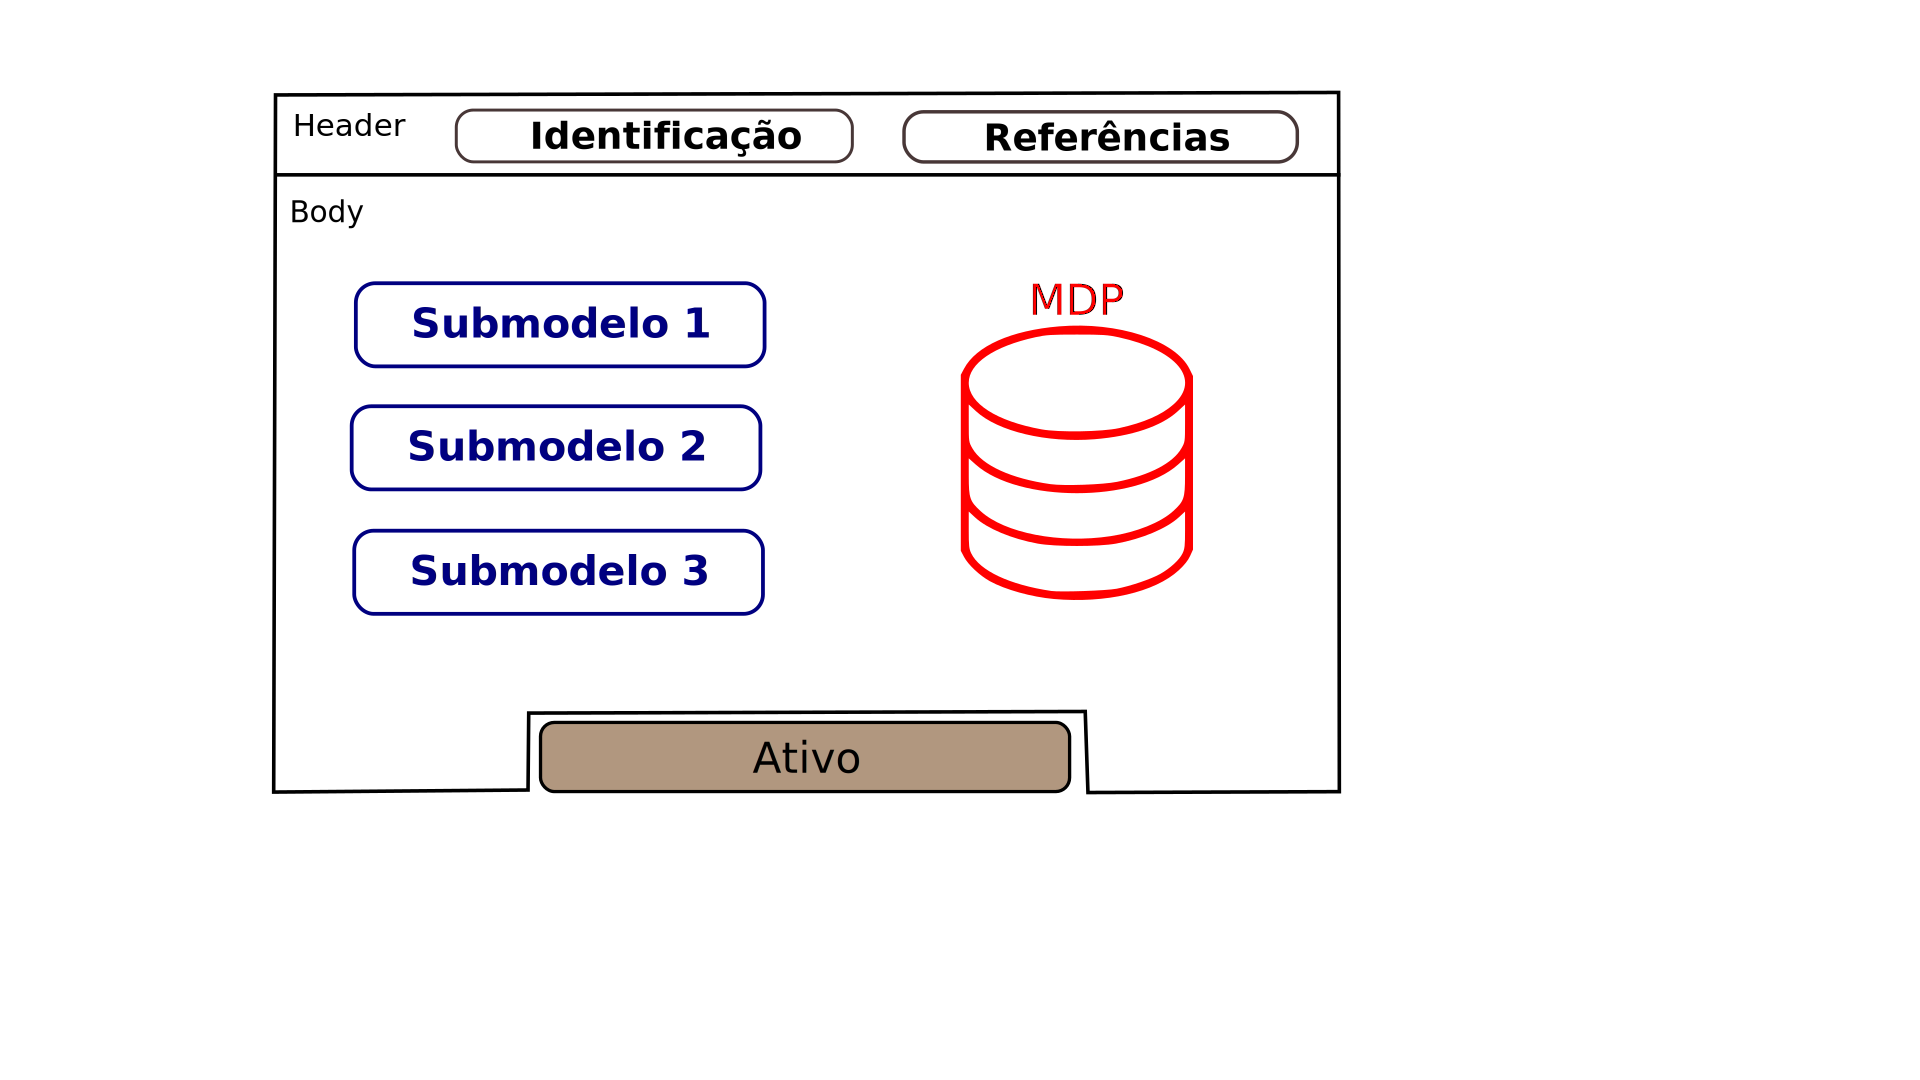
\includegraphics[width=1\textwidth]{submodelos.png}
		\fonte{\citeonline{bedenbender2017aasexamples} (adaptado).}
	\end{figure}

	No ambiente de manufatura baseado na I4.0, o produto descreve os requerimentos necessários para sua fabricação e então esses requerimentos são comparados com as descrições da funções das máquinas disponíveis. Portanto, a seleção de um ativo é otimizada, baseando-se nos requerimentos do produto e nas descrições das funções dos ativos.

\section{Memória digital do produto}

	Os produtos que são produzidos no cenário de Indústria 4.0 são equipados com a mémoria digital do produto (MDP). Por meio dessa memória podem ser acessadas e redistribuídas informações sobre o produto ao longo de toda a cadeia de valores.

	A MDP é alimentada e disponibilizada ao longo de todo o ciclo de vida do produto, podendo ser acessada por qualquer elo na cadeia de suprimentos (fabricante, distribuidor, varejista, consumidor). Mesmo no pós-venda, a MDP ainda se faz presente. O consumidor ainda pode ter acesso às informações dos produtos em cada ponto da cadeia de suprimentos e se beneficiar de serviços individuais que se acumulam na memória \cite{brandherm2011productmemory}.

	Nesse contexto, a MDP mantém informações relevantes de eventos ocorridos ao longo do ciclo de vida do produto a fim de fornecer serviços a todo o ambiente com o qual o produto se relaciona \cite{brandherm2011productmemory}.
	
	A MDP fornece também uma forma de rastreabilidade de produtos ao longo da cadeia de valores uma vez que pode armazenar informações geoespaciais do ativo ao longo do tempo.

\section{Arquitetura orientada a serviços (SOA)}
	
	Arquitetura Orientada a Serviços (SOA) é um estilo de projeto de software em que serviços são disponibilizados a outros sistemas por meio de protocolo de comunicação comum em uma rede \cite{bell2008soa}. Um serviço SOA é uma unidade de funcionalidade que pode ser fornecida/acessada remotamente. A SOA se destina a ser independente de fornecedores, produtos e tecnologias.
	
	Para quem consome um serviço SOA, a abordagem é como uma caixa preta, o que significa que o consumidor não não sabe ou não precisa estar ciente do funcionamento interno do serviço, sendo apenas o resultado do serviço relevante. Os serviços SOA representam uma lógica de fornecimento de resultados que possibilitam a abstração de problemas.
	
	Dentro do mundo da Indústria 4.0 e de sistemas produtivo, a SOA é uma abordagem que	traz novas perspectivas uma vez que se estabelece um conjunto de princípios para uma arquitetura de sistema autônomo e interoperável \cite{candido2009soa}, que tem por objetivo aumentar a eficiência, agilidade e produtividade de um sistema por meio da adoção generalizada do conceito de serviços. \cite{souit2013soa}.
	
	Os serviços SOA dentro do ambiente de manufatura encapsulam as funcionalidades necessárias, ocultando todas as heterogeneidades das partes do sistema, permitindo, desta forma, características de flexibilidade, confiabilidade e fácil implementação de	soluções \cite{groba2008soa}.
	
	A SOA dentro do meio industrial permite que um sistema atue como \textit{Middleware}, ou seja, uma camada ou componente de software que integra os diferentes aplicativos em um sistema. A \autoref{fig:middleware} ilustra como se dá a interconexão entre os elementos do sistema com e sem um \textit{middleware}.
	
	\begin{figure}[htb]
		\centering
		\caption{Interconexão entre os elementos do sistema com e sem um \textit{middleware}.}
		\label{fig:middleware}
		\includegraphics[width=1\textwidth]{middleware.png}
		\fonte{\citeonline{gosewehr2017middleware} (adaptado).}
	\end{figure}

	SOA está relacionado à ideia de uma Interface de Programação de Aplicação (Application Programming Interface - API), que é o conjunto de rotinas e padrões estabelecidos por um \textit{software} para a utilização das suas funcionalidades por aplicativos externos.
	
	Para se disponibilizar um serviço SOA, os Web Services (WSs) são a tecnologia mais adotada para
	implementar uma API \cite{souit2013soa}. Os WSs podem ser vistos como uma tecnologia padrão para facilitar a interoperabilidade, integração e reuso de componentes da aplicação, isto é, serviços.
	
	\subsection{Serviços Web}
	
	Um serviço da Web é uma interface que descreve uma série de operações acessíveis por meio de uma linguagem de descrição de serviços padronizada \cite{gottschalk2002webservices}. Um serviço da Web executa uma tarefa específica ou um conjunto de tarefas e retorna ao usuário o resultado da operação. Cada aplicação pode ter a sua própria linguagem, que é traduzida para uma linguagem comum, como um XML, JSON, CSV, etc.
	
	Por meio de WSs, as aplicações podem ser descritas, publicadas, localizadas e invocadas em uma rede de comunicação tipo www (World Wide Web) \cite{souit2013soa}.
	
	A arquitetura do Web Service é constituída por três atores básicos: o provedor, o repositório e o solicitante; e por três operações básicas: a publicação, a procura e a interação \cite{gottschalk2002webservices}. A \autoref{fig:componentes-webservice} ilustra os atores e a interação entre eles por meio das operações.
	
	Detalhadamente, os atores em um WS são:
	
	\begin{itemize}
		\item \textbf{Provedor de serviços}: Representa a plataforma que hospeda e fornece um determinado serviço, esta plataforma permite que clientes solicitem serviços e recebam suas respectivas respostas. O provedor de serviços é responsável também por fornecer uma descrição sobre o serviço prestado e publicar esta descrição em um repositório acessível pelo solicitante.
		
		\item \textbf{Repositório}: É uma plataforma acessível com a função de armazenar e fornecer a descrição sobre diversos WSs. Os WSs são descobertos pelo solicitante por meio do repositório para que assim possa decidir o serviço que melhor o atenda.
		
		\item \textbf{Solicitante de serviços}: É o ator que necessita de um determinado serviço e requisita a sua execução. O solicitante de serviço pode ser uma pessoa acessando um navegador ou uma aplicação realizando solicitações por meio de APIs.		
	\end{itemize}

	\begin{figure}[htb]
		\centering
		\caption{Componentes de um WS e operações.}
		\label{fig:componentes-webservice}
		\includegraphics[width=1\textwidth]{componentes-webservice}
		\fonte{\citeonline{kreger2001webservices} (adaptado).}
	\end{figure}
	
	Já as operações básicas em WS em detalhe são:
	
	\begin{itemize}
		\item \textbf{Publicação}: Publicação pelo provedor da descrição do serviço em um repositório para que o serviço se torne acessível a público e solicitantes possam localizá-lo. 
		\item \textbf{Busca}: Busca e recebimento da descrição de um serviço. O solicitante pode receber a descrição do serviço pelo provedor ou por meio do repositório.
		\item \textbf{Interação}: Comunicação direta entre solicitante e provedor para o fornecimento de serviços. Nesta fase, o solicitante se decide por um determinado serviço dentro os disponíveis no repositório e inicia uma interação com o provedor por meio de uma API.
	\end{itemize}
	
	As etapas de interação entre as entidades são representadas por meio de diagrama UML na \autoref{fig:uml-webservice}.
	
	\begin{figure}[htb]
		\centering
		\caption{Diagrama UML com os atores e interações em um WS.}
		\label{fig:uml-webservice}
		\includegraphics[width=1\textwidth]{uml-webservice}
		\fonte{\citeonline{booth2004webservice} (adaptado).}
	\end{figure}

	Os WSs se tornaram bastante atrativos, pois este modelo pode ser aplicado com tecnologias acessíveis ao solicitante, em particular XML e HTTP, que podem ser acessadas pela maioria dos navegadores convencionais. A disponibilização de serviços interativos na Web se tornou muito popular e com isso aparecem novos modelos de negócios como o SaaS (\textit{Software as a Service}), PaaS (\textit{Platform as a Service}), IaaS (\textit{Infrastructure as a Service}), etc.
	
	Dentro do mundo da Indústria 4.0 não é diferente. Ativos podem publicar suas funcionalidades em repositórios e executarem determinadas tarefas mediante solicitação por parte do solicitante, podendo assim serem classificados uma manufatura como um serviço (\textit{Manufacturing as a Service}) \cite{annunziata2019maas, nichols2020maas, siepen2019maas}.
	
	\subsection{Transferência Representacional de Estado}
	
	A Transferência Representacional de Estado (\textit{Representational State Transfer} - REST) é uma arquitetura de \textit{software} que define padrões para acesso e disponibilização de \textit{Web Services} (WSs). Os WSs que seguem o padrão REST são denominados \textit{RESTful Services}.
	
	A arquitetura REST possibilidade a interoperabilidade entre sistemas na Internet, pois permitem que os sistemas solicitantes acessem e manipulem representações textuais de recursos usando um conjunto uniforme e predefinido de operações sem estado \cite{ferris2004webservices}.
	
	Quando o HTTP é usado como protocolo de comunicação em um serviço REST, cada método do protocolo recebe um tipo de operação padrão do REST. A \autoref{tab:rest} mostra as possíveis operações em um RESTful Service e seu método HTTP correspondente, quando este protocolo é utilizado.
	

	\begin{table}[htb]
		\centering
		\footnotesize
		\caption{Possíveis operações em um \textit{RESTful Service}.}
		\label{tab:rest}
		\begin{tabulary}{\textwidth}{ |C|C|C|C| }
			\hline
			\textbf{Operação} &
			\textbf{Método HTTP} &
			\textbf{Resposta (item único)} &
			\textbf{Resposta (itens diversos)} \\

			\hline
			Criação &
			POST &
			201 (Criado) &
			Não aplicável. \\
			
			\hline
			Leitura &
			GET &
			200 (OK) &
			200 (OK) ou 404 (Não encontrado) \\
			
			\hline
			Atualização &
			PATCH &
			405 (Não permitido) &
			200 (OK), 204 (Sem conteúdo) ou 404 (Não encontrado) \\
			
			\hline
			Exclusão &
			DELETE &
			405 (Não permitido) &
			200 (OK) ou 404 (Não encontrado) \\[5mm]
			
			\hline
		\end{tabulary}
		\fonte{\cite{fielding2000architecture} (adaptado).}
	\end{table}

\chapter{Arquitetura para compartilhamento de informações do ativo}
\label{cha:arquitetura}
	
	A elaboração de uma arquitetura comum para o compartilhamento de informações do ativo é essencial para que haja consistência e interoperabilidade entre os membros da Cadeia de Suprimentos (CS) adotando este sistema.
	
	Este capítulo tem o objetivo de apresentar detalhes da arquitetura proposta baseada em \textit{Web Services} (WS) nos modelos de uma arquitetura orientada a serviços (SOA) compatível com Componentes I4.0 para o compartilhamento de informações do ativo ao longo da CS. A fim de simplificação do texto, os \textit{Web Services} serão mencionados apenas como ``serviços''.
	
	Neste capítulo é apresentado também o mapeamento dos componentes desta arquitetura dentro do eixo camadas do RAMI4.0.
	
\section{Componentes e operações de serviços dos AASs}

	Os serviços no escopo desta arquitetura são representações das funcionalidades dos Componentes I4.0 e são fornecidos e consumidos entre \textit{Asset Administration Shells} (AASs).
	
	A lógica de fornecimento e consumo de serviços proposta para a I4.0 segue os moldes de um \textit{Web Service} explicado na \autoref{sec:webservices}, apresentando os componentes e operações (vide \autoref{fig:webservice-componentes}) adaptados ao AAS.
	
	Esta arquitetura envolve três componentes (atores) básicos: O AAS cliente, o AAS servidor e o AAS repositório; e três operações: publicação, busca e interação.

	Os serviços disponibilizados remotamente pelo AAS servidor escuta e responde solicitações de clientes por meio de uma determinada rede e porta. Os AAS clientes, por sua vez, consomem o serviço disponibilizado pelo servidor por meio de solicitações.
	
	Nesta seção são apresentados detalhes sobre os componentes e operações necessárias para o fornecimento serviços no mundo conectado da I4.0.
	
\subsection{Componentes}

	Os componentes da arquitetura e suas inter-relações são apresentados na \autoref{fig:aas-ws}.
	
	\begin{figure}[htb]
		\centering
		\caption{Componentes e operações do WS.}
		\label{fig:aas-ws}
		\includegraphics[width=0.7\textwidth]{aas-ws}
		\fonte{O autor.}
	\end{figure}

	De maneira sucinta, os componentes são descritos da seguinte forma: ``O AAS Servidor'' é a parte que possui um serviço a oferecer para os demais AASs no mundo conectado, o ``AAS Cliente'' é a parte que necessita de um serviço e que age ativamente para receber este serviço e o ``AAS Repositório'' é a parte que armazena informações sobre descrições de diversos serviços.
	
	A \autoref{tab:componentes-ws} lista os componentes da arquitetura para a I4.0 e suas respectivas descrições detalhadas.
	
	\begin{table}[htb]
		\centering
		\caption{Componentes da arquitetura para a I4.0.}
		\label{tab:componentes-ws}
		\begin{tabular}{p{3cm}p{12cm}}
			\hline
			\textbf{Componente}
			& \textbf{Descrição} \\ 
			
			\hline
			AAS Servidor
			& O AAS Servidor é a conexão direta com o ativo. Este AAS extrai as informações sobre seu ativo para sua própria MDP para que assim possam ser disponibilizadas na rede. Cada submodelo do AAS representa um conjunto de informações e serviços semelhantes agrupados. \\
			
			\hline
			AAS Cliente
			& O AAS Cliente é a parte que irá consumir as informações disponibilizadas pelo AAS Servidor. O cliente representa cada uma das partes envolvidas na cadeia de suprimentos. Pode representar uma instituição, uma pessoa física ou até mesmo uma outra máquina/produto. \\
			
			\hline
			AAS Repositório
			& O repositório é o componente que recebe, armazena e disponibiliza informações de descrição sobre todos os serviços disponíveis no mundo conectado. O AAS recebe operações de ``publicação'' por parte do AAS Servidor e operações de ``busca'' por parte do AAS Cliente. O Repositório não atua como canal de comunicação entre AAS Cliente e Servidor, mas apenas fornece informações necessárias para que ambos os AAS possam se comunicar diretamente por meio da operação de ``interação''. \\
			
			\hline
		\end{tabular}
		\fonte{O autor.}
	\end{table}
	
	Neste modelo, a descrição dos serviços disponíveis nos submodelos de cada AAS é armazenada em um repositório comum, onde todos os AASs disponíveis no mundo conectado na I4.0 poderiam se tornar visíveis. A função do repositório é armazenar uma descrição dos serviços disponíveis e não o serviço em si. O serviço é fornecido pelo próprio AAS Servidor que o disponibilizou, servindo o repositório apenas como um elemento para a descoberta de serviços.

	Cada AAS pode atuar tanto como um fornecedor de serviços (servidor), quanto como um solicitante de serviços (cliente), ou como ambos. Sempre usando o repositório como meio para a publicação ou busca dos serviços.

\subsection{Operações}

	As operações de serviços de AASs e suas inter-relações com os componentes são mostradas por meio dos arcos na \autoref{fig:aas-ws} e suas descrições detalhadas são apresentadas na \autoref{tab:operacoes-ws}
	
	\begin{table}[htb]
		\centering
		\caption{Operações do WS para a I4.0.}
		\label{tab:operacoes-ws}
		\begin{tabular}{p{3cm}p{12cm}}
			\hline
			\textbf{Operação}
			& \textbf{Descrição} \\ 
			
			\hline
			Publicação
			& Ação tomada pelo AAS Servidor sempre que este componente queira anunciar um serviço para que possa ser descoberto. Nesta operação, o AAS Servidor envia uma lista de seus serviços ofertados e a descrição de cada um desses serviços. Esta lista é recebida e armazenada pelo AAS Repositório, que a disponibiliza para acesso público. \\
			
			\hline
			Busca
			& Ação tomada pelo AAS Cliente sempre que este precisa consultar serviços de seu interesse. Nesta operação o AAS Cliente faz uma solicitação ao AAS Repositório com os parâmetros que definem o tipo e as restrições do serviço desejado. A operação de busca engloba também o fluxo contrário de informações, que é o envio da resposta da solicitação do AAS Repositório para o AAS Cliente. \\
			
			\hline
			Interação
			& Ação tomada pelo AAS Cliente sempre que este deseja invocar um serviço. O AAS Cliente estabelece uma conexão direta com o AAS Servidor e consome o determinado serviço solicitado. A operação de interação normalmente é feita após o recebimento da lista de descrição de serviços por parte do AAS Repositório, porém a interação pode ser feita diretamente caso o AAS Cliente já possua informações necessárias para o estabelecimento da conexão.  \\
			
			\hline
		\end{tabular}
		\fonte{O autor.}
	\end{table}

	Para cada uma das operações, deve ser definido também o WSD (\textit{Web Services Description}), documento o qual estabelece os padrões de comunicação suportados pelo AAS Servidor como, por exemplo, o padrão REST ou o padrão SOAP; e especifica como acessar e quais as operações ou métodos estão disponíveis no serviço. 
	
	Quando o AAS atua como Servidor, este publica a descrição de seus serviços no repositório por meio de uma API (\textit{Application Programming Interface}) definida no WSD. Quando como Cliente, o AAS busca no repositório um serviço desejado e recebe uma lista de opções de serviços com suas respectivas descrições. Assim, o serviço mais adequado pode ser selecionado.
	
	Uma vez definido o serviço a ser consumido, o AAS Cliente estabelecerá a conexão direta com o AAS Servidor por meio de algum dos padrões suportados, utilizando os detalhes contidos na descrição do serviço para localizar, contactar e invocar o serviço.	
	
	A \autoref{fig:pfs-ws} apresenta um diagrama PFS (\textit{Production Flow Schema}) (vide \autoref{sec:modelagem}), com o fluxo de ocorrência das operações básicas no WS para a I4.0.
	
	\begin{figure}[htb]
		\centering
		\caption{Diagrama PFS das operações do WS.}
		\label{fig:pfs-ws}
		\includegraphics[width=1\textwidth]{pfs-ws}
		\fonte{O autor.}
	\end{figure}
	
	Os serviços fornecidos por um AAS são diversos. Entretanto, neste trabalho serão tratados com ênfase aqueles serviços que têm como objetivo o compartilhamento de informações sobre o ativo que possam agregar valor ao produto ao longo de sua cadeia de suprimentos. Ou seja, os serviços que extraem informações da MDP do AAS e as fornecem, mediante autenticação, às partes solicitantes ao longo da cadeia de suprimentos.

\section{Estrutura do AAS}

	Nesta proposta de arquitetura de WS, o conceito de Memória Digital do Produto (MDP) é inserido dentro da Indústria 4.0 com o objetivo de se agregar valor ao produto por meio da possibilidade de acesso a informações sobre o ativo entre parceiros ao longo da cadeia de valor.
	
	Nesta seção são apresentados os detalhes sobre uma possível estruturação do AAS para que seja compatível com a proposta de compartilhamento de informações por meio de WSs.
	
	\subsection{Integração da MDP ao AAS}
	
	A MDP precisa ser integrada ao AAS para que possa ter a estrutura necessária para que seus dados sejam disponibilizados ao mundo conectado da I4.0. A MDP em um AAS corresponde à organização dos dados do ativo, ao gerenciamento desses dados e às funções básicas aplicadas em cima desses dados. A MDP é uma \textit{view}, ou seja, ela replica e agrega as informações referentes a cada um dos submodelos de um AAS e as organiza de forma a poderem ser facilmente disponibilizadas por meio de WSs.
	
	Como a MDP é parte integral do AAS, que representa a parte virtual do ativo, esta pode ser fornecida em qualquer meio digital, inclusive em plataformas de serviços de computação em nuvem. Estas plataformas específicas suportam o armazenamento de grandes quantidades de dados, assim como podem assegurar uma alta capacidade de processamento de requisições de serviços.
	
	As informações contidas na MDP devem ser estruturadas de tal forma que simplifique a interpretação destes dados do lado do cliente. Para isso, metamodelos devem ser estabelecidos a fim de se criar moldes sobre os quais os dados devem ser estruturados.
	
	\citeonline{bader2019aas} estabelece padrões de metamodelos para a implementação de submodelos no AAS, porém não aborda um possível repositório de serviços e o armazenamento de descrições de serviços. A \autoref{tab:mdp-repositorio} traz uma proposta de metamodelo para a MDP do AAS Repositório para o armazenamento de descrições de serviços.
	
	\begin{table}[htb]
		\centering
		\caption{Proposta de metamodelo para a MDP do repositório.}
		\label{tab:mdp-repositorio}
		\begin{tabular}{p{3cm}p{12cm}}
			\hline
			\textbf{Propriedade}
			& \textbf{Descrição} \\ 
			
			\hline
			ID do AAS servidor
			& Tem a função de distinguir exclusivamente os AASs provedores de serviços e todos seus elementos \cite{adolphs2016structure} no mundo conectado da I4.0. Alguns tipos possíveis de identificadores são \cite{bader2019aas}: IRDI, IRI e UUID. O ID do AAS servidor é uma referência ao AAS Repositório e a todos os demais AASs que solicitarem a descrição dos serviços. \\
			
			\hline
			ID do serviço
			& Identificação exclusiva do serviço para a sua identificação única entre todos os repositórios. O ID do serviço pode ser derivado do próprio ID do AAS servidor com identificações extra do ID dentro do AAS (E.g., ID\_MODELO.SERVIÇO\_001). \\
			
			\hline
			Descrição do AAS provedor
			& Breve descrição sobre o AAS servidor e suas funções. \\
			
			\hline
			Protocolos de comunicação e padrões de API
			& Definição dos protocolos de comunicação suportados pelo fornecedor daquele serviço, como, por exemplo, HTTP, MQTT, etc; assim como as especificações do padrão para a comunicação via API como, por exemplo, REST, SOAP, GraphQL, etc.   \\
		
			\hline
			Formato de intercâmbio
			& Formato de arquivo de intercâmbio de informações. Ex.: json, xml, yaml, aasx, etc.  \\
			
			\hline
			\textit{Timestamp} da inserção do serviço no repositório
			& Data e hora de inserção do serviço ao repositório. \\
			
			\hline
			Indicação de disponibilidade
			& Chave booleana indicando se o AAS servidor atualmente suporta requisições. Esta propriedade pode estar desatualizada caso o AAS Servidor sofra uma falha de comunicação. Em outros casos, o AAS Servidor pode voluntariamente indicar ao repositório que temporariamente não processará solicitações de serviços. \\
			
			\hline
			Quality of Service (QoS)
			
			& A métrica de qualidade de serviço (QoT) fornece indicadores sobre a qualidade do serviço prestado por um determinado AAS. O tempo médio de resposta do serviço baseado no tempo de resposta observado por diversas requisições executadas e a disponibilidade do AAS quando solicitado são índices que contribuição do QoS. Um índice para serviços de qualidade mais subjetiva pode ser criado baseado em avaliações de AAS Clientes que já consumiram o serviço.\\
			
			\hline
			Descrição do serviço
			& Descrição sobre o funcionamento do serviço juntamente com o tipo de resposta esperado.  \\			
			\hline
		\end{tabular}
		\fonte{O autor.}
	\end{table}
	
	A \autoref{tab:mdp-repositorio} é uma lista não exaustiva das propriedades necessárias para o armazenamento de um serviço, ela apenas apresenta uma ideia sobre os tipos de chaves básicas necessárias para identificação e invocação de um serviço na rede.
	
	O AAS Cliente na operação de busca fará uma requisição ao repositório ou a uma lista de repositórios e receberá (de cada um dos repositórios) por meio de uma API a lista de serviços com uma estrutura de dados contendo os atributos chave-valor mencionados na \autoref{tab:mdp-repositorio}.
	
	Já o metamodelo da MDP do AAS servidor possuirá uma estrutura diferente, uma vez que deverá possuir as funções de agregação necessárias para a geração de alguns atributos. Uma proposta de metamodelo para a MDP do AAS servidor é apresentada na \autoref{tab:mdp-servidor}.
	
	\begin{table}[htb]
		\centering
		\caption{Proposta de metamodelo para a MDP do servidor.}
		\label{tab:mdp-servidor}
		\begin{tabular}{p{4cm}p{11cm}}
			\hline
			\textbf{Propriedade/Função}
			& \textbf{Descrição} \\ 
			
			\hline
			ID do serviço
			& Identificação exclusiva do serviço para a sua identificação única entre todos os repositórios. \\
			
			\hline
			Extração de dados dos submodelos
			& Função que retorna os dados solicitados pelo serviço. \\
			
			\hline
			Organização dos dados
			& Funções de estruturação dos dados ao formato solicitado pelo serviço, nesta fase pode haver também funções de limpeza dos dados brutos extraídos dos submodelos. \\
			
			\hline
			\textit{Quality of Service} (QoS)
			& Função para cálculo e armazenamento do índice de qualidade de serviço (QoS) com base em métricas sobre serviços já prestados e avaliações de AAS clientes que já consumiram o serviço. \\
			
			\hline
			Atualização da descrição do serviço no repositório
			& Função que envia ao repositório da empresa a descrição atualizada dos serviços. \\
			
			\hline
			Repositório
			& Referência ao repositório da empresa onde o ativo se encontra. \\			
			\hline
		\end{tabular}
		\fonte{O autor.}
	\end{table}
	
	A \autoref{tab:mdp-servidor}, assim como os metamodelos da MDP do Repositório (\autoref{tab:mdp-repositorio}), faz uma listagem não exaustiva de suas propriedades, sendo possível a inserção de novas funcionalidades adicionais na implementação do AAS. O metamodelo proposto na tabela se relaciona às funções da MDP em gerar a descrição dos serviços. Além desta atividade, a MDP possui as funções convencionais de armazenamento e gerenciamento dos dados dos submodelos.
	
	Com a MDP, o AAS servidor será, portanto, o único responsável pela geração e atualização de todos os metadados referentes aos serviços de seu AAS.

	
	\subsection{Detalhamento das partes do AAS}

	Nesta subseção é apresentada uma proposta de detalhamento dos elementos de um AAS contendo todas as partes necessárias para a implementação da arquitetura de compartilhamento de serviços baseada no RAMI4.0. 
	
	A estrutura proposta do AAS é baseda em \citeonline{bader2019aas}, que estabelece a divisão do AAS em submodelos e o divide em duas partes: o cabeçalho (\textit{header}) e o corpo (\textit{body}).
	
	O cabeçalho na estrutura proposta terá a função de providenciar informações públicas sobre o ativo que o identifiquem minimamente e que forneça uma descrição sobre seus serviços oferecidos. O cabeçalho deverá conter informações que podem ser acessadas sem a necessidade de autenticação, como, por exemplo, seu identificador único universal (UUID - \textit{Universal Unique IDentifier}), o modelo e fabricante do ativo. O cabeçalho deverá conter também a descrição dos serviços fornecidos por seus submodelos. A descrição dos serviços é enviada ao repositório ou pode ser também consultada diretamente pelo AAS solicitante.
	
	A descrição de cada serviço no cabeçalho deverá conter também referências ao próprio AAS como forma de referência para que, assim, o AAS Cliente possa localizar, contactar e invocar o serviço ofertado.
	
	O cabeçalho não terá a função de fornecer uma ficha técnica detalhada, mas apenas uma caracterização abstrata do ativo. O cabeçalho deverá necessariamente conter o UUID do AAS, sem o UUID o AAS se torna inacessível para qualquer uma das partes da cadeia de suprimentos.
	
	Dentro dos moldes da estrutura proposta, o corpo (\textit{body}) de um AAS fornece as informações e funcionalidades sensíveis sobre o ativo, que podem ser acessadas mediante autenticação. As funcionalidades dos ativos são agrupadas em forma de submodelos, conforme estabelecido em \citeonline{bader2019aas, adolph2018roadmap, bedenbender2017aasexamples}, que são unidades de agrupamento de funcionalidades semelhantes, como propriedades, serviços e demais regras de negócio do ativo. Os dados do ativo são armazenados nos próprios submodelos, enquanto a MDP (que também está contida no corpo do AAS) extrai e organiza as informações dos submodelos de forma a estruturá-las para serem diretamente fornecidas ao serviço.
	
	O corpo do AAS representa a carga útil (\textit{payload}) do AAS, pois é a porção de informação que é de fato relevante para o cliente que consumirá os serviços ofertados.
	
	A estrutura de um AAS compatível com a arquitetura orientada a serviços proposta é apresentada na \autoref{fig:estrutura-aas}.
	
	\begin{figure}[htb]
		\centering
		\caption{Estrutura do AAS com seus submodelos e a MDP.}
		\label{fig:estrutura-aas}
		\includegraphics[width=0.7\textwidth]{estrutura-aas}
		\fonte{O autor.}
	\end{figure}

	Os dados contidos nos submodelos, quando processados pela MDP, fornecem informações úteis sobre o ativo e agregam valor ao mesmo. Além disso, novos modelos de negócio surgem sob os dados gerados pelo ativo.
	
	Neste trabalho é dado enfoque aos submodelos que se relacionam a informações sobre o produto que sejam de interesse a qualquer uma das partes ao longo da cadeia de suprimentos e que possam ser lidos ou escritos por meio dos WSs. Alguns exemplos desse tipo de submodelo podem incluir: a ficha técnica detalhada do ativo, submodelos de histórico de leitura de sensores, histórico de leitura de geolocalização (GPS), histórico de padrões de uso, etc.


\section{Fluxo de fornecimento de serviços}

	As etapas para o fornecimento de serviços na I4.0 segue um fluxo padrão. Os submodelos agregam informações semelhantes que podem ser lidas ou escritas por qualquer uma das partes ao longo da CS mediante autenticação.
	
	Um fluxo de leitura/escrita de dados pode ser exemplificado com uma CS simples contendo três membros: um fabricante, um distribuidor e um consumidor; cada membro da CS é AAS Cliente diferente. O fabricante cria o produto, que será o AAS Servidor, e define a estrutura de seu AAS e seus submodelos necessários, três submodelos são definidos: submodelo ``Geolocalização'', submodelo ``Sensores'' e submodelo ``Documentação''. Ao longo do ciclo de vida do produto, os membros da CS (fabricante, distribuidor e consumidor) podem interagir com esses submodelos, fazendo sua leitura para o caso dos submodelos de geolocalização e sensores, e podendo fazer a leitura e/ou escrita para o caso do submodelo de documentação.
	
	A \autoref{fig:webservice-multielo} demonstra este cenário mencionado com o fluxo de operações básicas do WS em funcionamento. Neste exemplo, o AAS de um produto \textbf{(a)} mantém contato com o AAS da empresa do fabricante \textbf{(b)}, com o AAS da empresa do distribuidor \textbf{(c)} e com o AAS do consumidor final \textbf{(d)}, fornecendo o serviço de consulta de informações de diferentes submodelos para cada um dos solicitantes. 	
	
	\begin{figure}[htb]
		\centering
		\caption{Exemplificação das operações de publicação e busca com múltiplos clientes.}
		\label{fig:webservice-multielo}
		\includegraphics[width=0.8\textwidth]{webservice-multielo}
		\fonte{O autor.}
	\end{figure}

	Na \autoref{fig:webservice-multielo} são mostrados os três modelos dos AAS Produto: Submodelo ``geolocalização'' \textbf{(e)}, submodelo ``sensores'' \textbf{(f)} e submodelo ``documentação'' \textbf{(g)}. Os serviços de todos os submodelos disponíveis são mapeados pelas funções da MDP \textbf{(h)} e, assim, é gerada uma lista de descrições de serviços \textbf{(i)}. Esta lista de descrições de serviços é publicada \textbf{(j)} no repositório.
	
	O repositório \textbf{(k)} recebe a descrição de serviços do AAS Produto e as disponibiliza para consulta. O repositório receberá também listas de descrição de serviços de diversos outros AASs.
	
	Os AAS Clientes fazem a busca \textbf{(l)} no repositório. As buscas são feitas com parâmetros a fim de se restringir qual tipo de serviço aquele cliente pretende consumir, podendo-se restringir a busca, inclusive, ao serviço de um AAS específico, identificando-o por meio de seu UUID.
	
	Cada AAS Cliente (Fabricante, Distribuidor ou Consumidor), portanto, realiza a consulta ao AAS Repositório com os seus parâmetros de interesse e recebe a resposta com descrições detalhadas sobre os serviços disponíveis e informações para localizar, contactar e invocar estes serviços.
	
	O próximo passo após o recebimento da resposta do repositório é a decisão interna de cada AAS Cliente sobre qual serviço selecionar. Uma vez definido, o AAS Cliente estabelece uma comunicação direta com o AAS Servidor (produto) para o consumo do serviço selecionado.
	
	Este é um exemplo de consulta única. Em aplicações reais, o cliente normalmente invocaria o serviço de diversos AAS Servidores ao mesmo tempo, como, por exemplo, um fabricante solicitando informações de todas as máquinas de um modelo específico que foram vendidas a clientes espalhados pelo mundo para se realizar análise de dados a fim de se fazer uma manutenção preditiva por meio da identificação de potenciais falhas. Tal exemplo é demonstrado na \autoref{fig:webservice-multiproduto}.
	
	\begin{figure}[htb]
		\centering
		\caption{Exemplificação das operações de publicação e busca com múltiplos produtos.}
		\label{fig:webservice-multiproduto}
		\includegraphics[width=1\textwidth]{webservice-multiproduto}
		\fonte{O autor.}
	\end{figure}

	
	A \autoref{fig:webservice-multiproduto} demonstra a situação de uma consulta de um AAS Cliente em múltiplos produtos. Neste exemplo, cada AAS Produto (\textbf{a}, \textbf{b} e \textbf{c}) realiza uma operação de publicação (\textbf{f}) no AAS Repositório (\textbf{e}). 
	
	O AAS Servidor (Fabricante) (\textbf{d}) por sua vez faz uma busca no AAS Repositório especificando os parâmetros que restrinjam a pesquisa a somente determinados modelos de produtos e recebe como resposta todas as descrições dos serviços que correspondem aos critérios de busca.	
	
	Todas as atividades de invocação de serviços na fase de interação são feitas mediante autenticação. É responsabilidade das funções da MDP realizar a autenticação ou bloqueio dos serviços disponíveis de acordo com as políticas de acesso de cada AAS.
	
	É importante notar que no mundo da I4.0 todo ativo é englobado por um AAS e se torna um Componente I4.0. Como o repositório detém informações e funções que agregam valor ao negócio, este pode também ser considerado um ativo e, portanto, possui o seu próprio AAS, que é responsável por toda a parte virtual deste ativo.
	
\section{Mapeamento das operações no RAMI4.0}
	
	Segundo \citeonline{iec2017rami}, o RAMI4.0 fornece uma visão estruturada dos principais elementos de um ativo usando um modelo de níveis composto por três eixos. Desta forma, inter-relações complexas podem ser divididas em seções menores e mais gerenciáveis, combinando os três eixos para representar cada aspecto relevante do estado do ativo em cada ponto de seu ciclo de vida.
	
	Esta seção tem o objetivo de mapear as operações do WS para dentro das camadas do RAMI4.0 de forma a representar todas as etapas do fluxo de informações em um modelo unificado.
	
	O mapeamento para o RAMI4.0, que é uma arquitetura de referência para a I4.0, contribui para facilitar a execução de implementações de conceitos de I4.0 uma vez que estabelece um padrão de arquitetura que deve ser adotado por todos, garantindo a interoperabilidades entre os sistemas.

\subsection{Descrição das camadas do RAMI4.0}

	Na \autoref{sub:rami4} foram apresentados os detalhes do RAMI4.0 e o detalhamento de cada nível do eixo Camadas com suas funções gerais. Nesta subseção é apresentada cada camada com enfoque para suas funções específicas para as operações em um WS.

	A camada mais inferior, \textbf{Ativo} é onde estará o elemento real do Componente I4.0 (C4.0) como, por exemplo, máquinas, sensores, pessoas, etc; e qualquer outro elemento, físico ou não, que represente valor ao negócio. O ativo será a fonte de dados, os quais serão compartilhados por meio de serviços para as partes ao longo da cadeia de suprimentos.
	
	Para o compartilhamento de informações do produto no mundo I4.0, os dados a serem extraídos do ativo são estrategicamente selecionados como o objetivo de reunir somente os dados que possam agregar valor ao próprio ativo. Assim, estes dados selecionados são extraídos do ativo e repassados às camadas superiores até que cheguem na camada Informação, onde são armazenados nos submodelos.
	
	Cada elemento desta camada, os ativos, deve possuir meios de comunicação e identificadores únicos (UUID), para permitir o seu monitoramento e supervisão dos dispositivos de controle por meio do AAS \cite{adolphs2015rami}.
	
	Na arquitetura orientada a serviços, três tipos de ativos básicos podem ser elencados: o produto, que é a fonte de dados e fornecedor dos serviços (servidor); as empresas ou pessoas, que são os clientes que consomem as informações da MDP do produto e também podem alterá-la; e as descrições dos serviços (WSD), que é o ativo encapsulado pelo C4.0-Repositório, responsável por garantir a visibilidade de um produto na cadeia de suprimentos.
	
	Na camada \textbf{Integração} estão as funcionalidades responsáveis pela virtualização de todos os ativos da camada inferior \cite{adolphs2015rami}. Ela representa a ponte para a troca de informações entre o mundo real e o virtual.
	
	Na arquitetura proposta para o compartilhamento de informações do ativo, esta camada está presente no CI4.0-Servidor, pois é dele que serão extraídos os dados desde o ativo até as camadas superiores. Tanto o C4.0-Cliente quanto o C4.0-Repositório operam primariamente nas camadas virtuais, porém também possuem a camada Integração, que faz a conexão com a empresa e o WSD, respectivamente. Esta camada adotará alguma tecnologias para a transferência de dados por meio físico como, por exemplo, o Wi-Fi, Ethernet, 5G, Bluetooth, etc.
	
	A camada \textbf{Comunicação} estabelecerá o protocolo de comunicação OPC UA para o C4.0-Servidor se comunicar com os demais C4.0s dentro da própria empresa (integração vertical).
	
	Para a arquitetura de compartilhamento de informações de ativos, não haverá comunicação entre C4.0s dentro da própria empresa uma vez que todas as operações de um WS (publicação, busca e interação) ocorrem entre componentes de organizações distintas. Ainda assim esta camada é necessária uma vez que ela define também os padrões de comunicação entre as camadas de um mesmo AAS.
	
	%É feito o pré-processamento de dados nesta fase, ou seja, antes de ser enviado para a camada Informação, onde será salvo nos submodelos. O pré-processamento dos dados inclui a remoção de redundâncias, duplicidades e remoção de \textit{outliers}.

	%Portanto, esta camada estabelece os protocolos de comunicação entre AASs dentro da mesma empresa (integração vertical), como os protocolos de comunicação entre AASs de diferentes empresas (integração horizontal). 

	A camada de \textbf{Informação} é onde os dados são de fato armazenados. Para isso, modelos de estrutura de Banco de Dados (BD) são definidos de acordo os tipos de dados e suas aplicações. Alguns exemplos de estrutura de dados incluem: BDs relacionais (e.g., MySQL, Postgres, SQLite) \cite{morris2017relationaldatabase} e demais BDs NoSQL como os orientados a documentos (e.g., MongoDB, CouchDB), os do tipo chave-valor (e.g., Redis, DynanoDB), os de armazenamento em coluna ampla (e.g., Cassandra, HBase) e os baseados em grafos (e.g.,Neo4j, JanusGraph) \cite{schaefer2019nosql}.
	
	Desta forma, esta camada é responsável por gerar e armazenar o WSD dos serviços oferecidos por cada C4.0-Servidor. Além disso, esta camada contém a parte da MDP que realiza a autenticação dos C4.0s solicitantes, ou seja, realiza o controle de acesso a suas informações.
	
	Na camada \textbf{Funcional} é onde ocorre toda a interação horizontal com C4.0s contidos no mundo conectado da I4.0. Esta camada é responsável pela integração horizontal entre as partes da cadeia de suprimentos de um produto. Os serviços são disponibilizados por meio da camada funcional, portanto é a interface entre os C4.0s de diferentes empresas.
	
	Esta camada deve definir o tipo de protocolo a ser utilizado para o fornecimento dos \textit{Web Services}, o protocolo HTTP é o mais comumente adotado para o fornecimento de WSs \cite{gruner2016restful}. Outros protocolos de aplicação também podem ser adotados como, por exemplo, o MQTT \cite{yokotani2016mqtt}.
	
	O fornecimento de serviços ao longo da cadeia de suprimentos é considerado uma integração horizontal uma vez que cada parte da CS representa uma organização diferente. Para o fornecimento e consumo desses serviços de compartilhamento de informações, devem ser definidas também as especificações da API, ou seja, o padrão de requisição e resposta para o fornecimento e consumo de serviços como, por exemplo, o padrão REST.
			
	A última camada, \textbf{Regra de Negócio}, é onde estão contidas as restrições legais e as políticas internas da empresa a serem aplicadas ao AAS \cite{adolphs2015rami}. No contexto da arquitetura de compartilhamento de informações do ativo baseada em \textit{Web Services}, esta camada conterá as restrições aplicadas sobre os serviços, como as políticas de privacidade de dados (E.g., restrições de acesso a determinados serviços) e as restrições legais de cada país.
	
	A regra de negócio estabelecerá quem na cadeia de suprimentos terá permissão para acessar quais informações do produto e quando. Um fabricante, por exemplo, terá acesso aos dados de padrões de uso de um produto somente sob a permissão do consumidor, o que representa uma regra nesta camada. Um distribuidor, por sua vez, só poderá ter acesso à localização do produto enquanto o produto estiver sob sua custódia.
	
	Outro ponto relevante desta camada para a arquitetura de compartilhamento de informações ao longo da CS são as condições legais de cada país, que criam restrições sobre o fornecimento de serviços, principalmente no aspecto de governança de dados.
	
	%Para os WSs, outra função importante desta camada é a orquestração dos serviços, que se refere ao gerenciamento dos serviços oferecidos. Quando os serviços são oferecidos em forma de contêineres, o orquestrador de serviços permite a escalabilidade da capacidade de trabalho, permitindo a invocação ou remoção de contêineres de acordo com a demanda de um determinado serviço. Alguns orquestradores de contêineres podem ser citados, como o Kubernetes, Docker Swarm e Apache Mesos \cite{redhat2020orchestration}.
	
	O conjunto de todas estas camadas representa um \textbf{Componente I4.0} (C4.0). Para cada tipo de operação relacionada a um componente, é necessário detalhar o fluxo de dados e de eventos acontecendo em cada uma das camadas. Este detalhamento permite que implementações de soluções I4.0 sejam facilitadas e garante que a criação dessas soluções por diversos desenvolvedores de sistemas resulte em sistemas que sejam interoperáveis, independentemente da tecnologia adotada.
	
	O \textbf{Componente I4.0} pode ainda ser mais detalhadamente especificado, identificando se o componente representa um produto em desenvolvimento ou uma instância de um produto já fabricado. Estes detalhes são cobertos pelo eixo Ciclo de Vida e Cadeia de Valor e considerações sobre este eixo envolvendo a arquitetura proposta baseada em WSs é apresentada no \autoref{cha:ciclo-de-vida}.
	
	A \autoref{fig:webservice-rami} apresenta os componentes da arquitetura de fornecimento de WSs dentro do eixo Camadas do RAMI4.0, que são:
	
	\begin{itemize}
		\item \textbf{Ativo}: Pessoas e empresas (cliente), produtos (servidor) e WSDs (repositório); 
		\item \textbf{Integração}: Virtualização das informações, protocolos de transferência de dados (Ethernet, 5G, Wi-Fi, etc); 
		\item \textbf{Comunicação}: Protocolos de comunicação vertical (OPC UA); 
		\item \textbf{Informação}: Controle de acesso / autenticação, análise de dados, armazenamento, descrição dos serviços (virtual);
		\item \textbf{Funcional}: Serviços de compartilhamento de informações, protocolos de comunicação horizontal (HTTPS, MQTT, etc), interface horizontal entre AASs; 
		\item \textbf{Regra de negócio}: Restrições legais, políticas de privacidade.
	\end{itemize}
	
	\begin{figure}[H]
		\centering
		\caption{Camadas do RAMI4.0 com os elementos da arquitetura.}
		\label{fig:webservice-rami}
		\includegraphics[width=0.7\textwidth]{webservice-rami}
		\fonte{O autor.}
	\end{figure}

\subsection{Operação de Publicação}

	A \autoref{fig:rami-publicacao} apresenta diagramas PFS do fluxo de atividades para a operação de publicação de um C4.0-Servidor em um C4.0-Repositório.
	
	\begin{figure}[htb]
		\centering
		\caption{Diagrama PFS da operação de publicação.}
		\label{fig:rami-publicacao}
		\includegraphics[width=1\textwidth]{rami-publicacao}
		\fonte{O autor.}
	\end{figure}

	Esta operação é iniciada pelo C4.0-Servidor, seguindo um fluxo de atividades estabelecido até chegar no ativo do C4.0-Repositório, os passos são detalhados a seguir:
	
	\begin{enumerate}
		
		\item As restrições legais e as políticas de privacidade para um determinado C4.0 são definidas e acessadas. Esta atividade adicionará restrições ao serviço a ser publicado. Estas restrições serão incorporadas à descrição de cada serviço a ser publicado.
		
		\item A geração da lista de descrições de serviços (WSD) é feita com base nos serviços disponíveis no C4.0-Servidor e nas restrições impostas na atividade anterior. Uma descrição de cada serviço ativo é gerada em um formato de intercâmbio padronizado.
		
		\item A MDP local componente armazena a lista de WSD nos submodelos.
		
		\item São definidos os protocolos de comunicação a serem utilizados na integração horizontal, assim como a especificação do padrão de requisição e resposta da API e o formato de intercâmbio de informações.
		
		\item A lista de WSD é enviada ao CI4.0-Repositório via API.
		
		\item O C4.0-Repositório recebe a lista de WSD no formato de intercâmbio definido. A descrição dos serviços nesta fase já contém todas as informações para a identificação do serviço e de seu componente correspondente.
		
		\item A lista de WSD é armazenada junto às demais descrições de serviços na MDP do C4.0-Repositório.
		
		\item São definidos os protocolos de comunicação vertical para a comunicação com as camadas inferiores.
		
		\item Os dados alimentam uma interface para comunicação com o ativo real.
		
		\item Os dados são escritos em disco.
	\end{enumerate}

\subsection{Operação de Busca}

	A operação de busca é dividida em duas partes: a requisição e a resposta. A requisição é a iniciativa do C4.0-Cliente para requerer a lista de WSD de um C4.0-Repositório. O fluxo de atividades da requisição em uma operação de busca é apresentado na \autoref{fig:rami-busca-requisicao}.
	
	Já a resposta da requisição em uma operação de busca é feita do C4.0-Repositório para o C4.0-Cliente e é apresentada na \autoref{fig:rami-busca-resposta}.
	
	\begin{figure}[htb]
		\centering
		\caption{Diagrama PFS da requisição em uma operação de busca.}
		\label{fig:rami-busca-requisicao}
		\includegraphics[width=1\textwidth]{rami-busca-requisicao}
		\fonte{O autor.}
	\end{figure}

	A operação de requisição para a busca de um serviço parte do C4.0-Cliente e segue um fluxo estabelecido até chegar ao C4.0-Repositório, esses passos são detalhados a seguir:
	
	\begin{enumerate}
		
		\item O processo de requisição começa com a definição por parte do ativo do C4.0-Cliente (pessoa ou empresa) da informação que se deseja consultar como, por exemplo, leituras de sensores, localização geográfica, manuais, etc. Essa definição pode ser manual, partindo da solicitação explícita de alguém, ou programática.
		
		\item A partir do tipo de informação a ser consultada, define-se os parâmetros de consulta, que representam o conjunto de restrições que estabelecem qual é exatamente o tipo de serviço que o AAS Cliente deseja consumir. Para os serviços que visam a extração de informações do ativo, os parâmetros representam, por exemplo, o ID do provedor de serviços, o horário e data de um determinado evento, uma filtragem por modelos específicos de um produto, etc.
		
		\item Os parâmetros de consulta alimentam uma interface para que a solicitação possa ser virtualizada e integrada ao AAS. Nesta atividade a intenção de solicitação de um serviço é virtualizada.
		
		\item São definidos os protocolos de comunicação vertical para a comunicação com as camadas superiores.
		
		\item A MDP local armazena os detalhes da solicitação em um registro de solicitações realizadas.
		
		\item São definidos os protocolos de comunicação a serem utilizados na integração horizontal, assim como a especificação do padrão de requisição e resposta da API e o formato de intercâmbio de informações.
		
		\item A requisição é enviada ao C4.0-Repositório via API.
		
		\item O C4.0-Repositório recebe a solicitação e a insere ao final da lista de solicitações para ser processada.
		
		\item A requisição é processada. Identifica-se nesta atividade se a requisição é válida e se ela contém todos os parâmetros necessários para a consulta.
		
		\item A MDP realiza a consulta à lista de WSDs utilizando os parâmetros de consulta estabelecidos.
		
		\item São definidos os protocolos de comunicação vertical para a comunicação com as camadas inferiores.
		
		\item Estabelece-se uma interface para a interação entre o AAS e seu ativo real.
		
		\item As informações solicitadas são lidas do disco e se tornam disponíveis para envio.
	\end{enumerate}

	Após a requisição, o C4.0-Repositório envia a resposta ao C4.0-Cliente. O fluxo de atividades da resposta é apresentada em diagramas PFS na \autoref{fig:rami-busca-resposta}.

	\begin{figure}[htb]
		\centering
		\caption{Diagrama PFS da resposta em uma operação de busca.}
		\label{fig:rami-busca-resposta}
		\includegraphics[width=1\textwidth]{rami-busca-resposta}
		\fonte{O autor.}
	\end{figure}

	Detalhadamente, a resposta do AAS Repositório segue o seguinte fluxo de atividades, começando pela disponibilização das informações reais do ativo repositório:
	
	\begin{enumerate}
		\item Os dados do ativo (WSD) são disponibilizados para consulta pelas camadas superiores.
		
		\item Os dados disponibilizados são virtualizados para a integração com o AAS.
		
		\item São definidos os protocolos de comunicação vertical para a comunicação com as camadas superiores.
		
		\item É realizada a consulta da lista de WSDs. Os resultados podem ser uma lista de serviços válidos, assim como podem conter mensagens de erro devido a solicitações inválidas ou buscas retornando zero correspondências.
		
		\item A lista de WSD é disponibilizada para acesso por parte da camada Funcional.
		
		\item São definidos os protocolos de comunicação a serem utilizados na integração horizontal, assim como a especificação do padrão de requisição e resposta da API e o formato de intercâmbio de informações.

		\item A resposta é enviada ao C4.0-Cliente via API.
		
		\item O C4.0-Cliente recebe a resposta contendo a lista de WSD em um formato de intercâmbio definido.
		
		\item Após a recepção da lista de serviços disponíveis, é feito o processamento para a definição do serviço mais adequado. Em consultas a serviços de compartilhamento de informações esta fase é simplificada, uma vez que os próprios parâmetros de consulta na requisição já definem o serviço ideal que o cliente busca. A seleção do serviço mais adequado é baseada nos parâmetros definidos na operação de requisição, que estabelecem os requisitos do serviço.
	\end{enumerate}

\subsection{Operação de Interação}

	A operação de interação é a fase final para o consumo de um serviço disponibilizado no mundo conectado da I4.0. Assim como a busca, a interação é divida em requisição e resposta. Primeiramente, o C4.0-Cliente faz uma requisição de consumo de um serviço com parâmetros e então a requisição é processada e respondida pelo C4.0-Servidor.
	
	 A \autoref{fig:rami-interacao-requisicao} apresenta o fluxo de atividades em uma requisição de um serviço e a \autoref{fig:rami-interacao-resposta} a resposta do serviço.
	
	\begin{figure}[htb]
		\centering
		\caption{Diagrama PFS da requisição de um serviço em uma operação de interação.}
		\label{fig:rami-interacao-requisicao}
		\includegraphics[width=1\textwidth]{rami-interacao-requisicao}
		\fonte{O autor.}
	\end{figure}

	A requisição de um serviço na operação de interação é iniciada pelo C4.0-Cliente e é enviada diretamente ao C4.0-Servidor usando a WSD fornecida pelo C4.0-Repositório. O fluxo de atividades para a requisição de um serviço é detalhada a seguir:
	
	\begin{enumerate}
		
		\item O processo de requisição começa com a definição exata sobre qual serviço de qual C4.0 será consumido. Caso a decisão seja feita manualmente, a intenção de requisição começa pelo ativo do C4.0-Cliente (pessoa ou empresa) com a seleção do serviço.
		
		\item Define-se os parâmetros da requisição de um serviço, que representam as opções obrigatórias ou opcionais para o detalhamento do serviço a ser consumido.
		
		\item Os parâmetros de consulta alimentam uma interface para que a requisição possa ser virtualizada e integrada ao AAS. Nesta atividade a intenção de interação é virtualizada.
		
		\item São definidos os protocolos de comunicação vertical para a comunicação com as camadas superiores.
		
		\item O processo de requisição pode iniciar diretamente da camada Informação por meio de uma decisão autônoma sobre o serviço mais adequado, sem a necessidade de uma tomada de decisão manual por parte de uma pessoa/empresa.
		
		\item A MDP local armazena os detalhes da requisição em um registro de requisições realizadas.
		
		\item São definidos os protocolos de comunicação a serem utilizados na integração horizontal, assim como a especificação do padrão de requisição e resposta da API e o formato de intercâmbio de informações.
		
		\item A requisição do serviço é enviada ao C4.0-Servidor via API.
		
		\item O C4.0-Servidor recebe a requisição e a insere ao final da lista de requisições para ser processada.
		
		\item A requisição é processada. Identifica-se nesta atividade se a requisição é válida e se ela contém todos os parâmetros necessários para o fornecimento do serviço.
		
	
	\end{enumerate}

	\begin{figure}[htb]
		\centering
		\caption{Diagrama PFS da resposta de um serviço em uma operação de interação.}
		\label{fig:rami-interacao-resposta}
		\includegraphics[width=1\textwidth]{rami-interacao-resposta}
		\fonte{O autor.}
	\end{figure}
	
	Após o recebimento e processamento da requisição de um serviço, o C4.0-Servidor deve fazer a extração e envio das informações do ativo. A resposta contendo as informações sobre o produto começa com a emissão de um evento no ativo. Esta informação percorre um fluxo padrão para que seja disponibilizada ao C4.0-Cliente por meio do serviço. Este fluxo de atividades mostrado na \autoref{fig:rami-interacao-resposta} é detalhado a seguir:
	
	\begin{enumerate}
		
		\item Um evento físico no mundo real é emitido.
		
		\item O evento fornece sinais físicos que podem ser medidos.
		 
		\item Os sinais físicos são interpretados e virtualizados. Nesta atividade é criado um correspondente virtual para o evento do ativo físico, ou seja, os dados são digitalizados e disponibilizados ao AAS.
		
		\item É definido o meio de transporte e o procolo de transferência de dados como, por exemplo, o Wi-Fi, Ethernet, 5G, etc.
		
		\item Os dados são devidamente transportados pelo meio e protocolo definidos até uma central de processamento.
		
		\item São definidos os protocolos de comunicação vertical para a comunicação com as camadas superiores.
		
		\item Os novos dados sobre o ativo são armazenados pela MDP nos submodelos junto aos demais dados já existentes.
		
		\item São definidas/acessadas as restrições legais e as políticas de privacidade para a autorização ou bloqueio do fornecimento do serviço.
		
		\item É feita a autenticação do C4.0-Cliente solicitante do serviço. Nesta atividade é verificado se o cliente possui autorização para consumir o serviço e consequentemente os dados que estão sendo solicitados.
		
		\item Após a autenticação, os dados são disponibilizados ao serviço.
		
		\item O serviço é executado e sua resposta é gerada. O serviço pode executar quaisquer operações sobre os dados atualizados sobre o ativo assim como sobre o histórico de registros antigos já disponíveis nos submodelos.
		
		\item São definidos os protocolos de comunicação a serem utilizados na integração horizontal, assim como a especificação do padrão de requisição e resposta da API e o formato de intercâmbio de informações.
		
		\item A resposta do serviço (fornecimento do serviço) é enviada via API.
		
		\item O C4.0-Cliente recebe a resposta do serviço no formato de intercâmbio definido.
		
		\item Os dados recebidos na resposta são processados.
		
		\item Opcionalmente a resposta e/ou resultados de processamento da resposta podem ser salvos na MDP local ou descartados.
	\end{enumerate}
	
\chapter{O ciclo de vida do produto na I4.0}
\label{cha:ciclo-de-vida}
	
	Este capítulo visa trazer discussões sobre o impacto do amplo compartilhamento da memória digital do produto ao longo da cadeia de suprimentos por meio de serviços na Indústria 4.0.
	
	São abordadas possíveis mudanças na curva de ciclo de vida do produto e o surgimento de novos modelos de negócio baseado em dados (\textit{data-driven}).
	
	Uma visão da MDP sobre o eixo ``Ciclo de Vida e Cadeia de Valor'' do RAMI4.0 é abordada, discutindo melhor o porquê e as atribuições dos AASs como ``tipos'' e como ``instâncias''.
	

\section{Ciclo de vida do produto no RAMI4.0}
	
	O modelo do RAMI4.0 apresenta um eixo de ciclo de vida generalizado, derivado da norma IEC 62890 \cite{adolphs2015rami}. O objetivo deste eixo é representar o ciclo de vida de um Componente I4.0 ao longo de toda a sua cadeia de valor.
	
	Os ``tipos'' estão presentes desde a concepção/conceitualização até os primeiros protótipos/testes. O ``tipo'' de um ativo é definido pelas suas propriedades e funcionalidades distintas. Todos os itens que são criados ao longo do projeto de um produto (e.g., desenhos em CAD, manuais, \textit{softwares}, etc) são incorporados ao ``tipo'' do ativo. Informações externas associadas ao ativo que são criadas ao longo de seu desenvolvimento como informações de \textit{marketing} também são incorporadas ao ``tipo''.
	
	As instâncias são criadas/produzidas/fabricadas com base nas informações de um ``tipo'' de ativo. Informações específicas sobre produção, logística, qualidade e testes são associadas à ``instância'' de um ativo. Nesta fase, os dados de uso são coletados e associados para então poderem ser armazenados na MDP e compartilhados com outros parceiros ao longo da cadeia de suprimentos. 
	
	O histórico completo do ciclo de vida do produto está associados à combinação entre ``tipo'' e a ``instância'' de um determinado produto. Estes dados podem ser aproveitados de forma inteligente para a geração de valor, gerando assim novos modelos de negócio.
	
	Os relacionamentos entre ``tipos'' e ``instâncias'' são cíclicos e possibilitam a retroalimentação de informações. Para os ativos de um produto, por exemplo, informações sobre seu uso e manutenção armazenadas na MDP podem auxiliar em melhorias no seu próprio processo de fabricação, além de ser fonte de dados para o desenvolvimento de novas versões aperfeiçoadas do mesmo produto, gerando um novo ``tipo''.
	
	Portanto, esse fluxo de informações entre ambas as fases de um produto são essenciais para a melhoria de seu próprio projeto. A \autoref{fig:aas-lifecycle} ilustra como ocorre a instanciação (criação de uma instância a partir de um tipo) e o uso da MDP das ``instâncias'' para a criação de novas versões de um ``tipo''.
	
	\begin{figure}[htb!]
		\centering
		\caption{Ciclo de vida do produto.}
		\label{fig:aas-lifecycle}
		\includegraphics[width=1\textwidth]{aas-lifecycle}
		\fonte{O autor.}
	\end{figure}

\section{Extração de informações pela MDP na fase ``tipo''}

	A extração de informações da MDP do produto auxilia no desenvolvimento de versões de ``tipos'' aprimoradas.

	Com os ciclos de vida do produto cada vez mais curtos e cadeias de logística cada vez mais complexas, explorar o registro informações do produto pode garantir uma posição competitiva de uma empresa comercial frente aos competidores.
	
	Além disso, a memória digital do produto abre novas possibilidades em relação ao combate à pirataria e falsificação de produtos, na proteção ao consumidor e na garantia de qualidade do produto \cite{wahlster2007digitalmemory}.
	
	A análise de dados da MDP possibilita o aprimoramento do ``tipo'' do produto das seguintes maneiras:
	
	\begin{itemize}
		\item Identificação e reparo de falhas de projeto;
		\item Adição de novas funcionalidades ao produto;
		\item Melhoria da experiência do cliente/operador com o produto;
		\item Geração de indicadores de sustentabilidade.
	\end{itemize}

	A \autoref{tab:produto-tipo} exemplifica possíveis informações e seus respectivos submodelos que agregam valor ao produto por meio da geração de novos ``tipos''.
	
	\begin{table}[htb]
		\centering
		\caption{Possíveis informações e respectivos submodelos para o aprimoramento do projeto do produto.}
		\label{tab:produto-tipo}
		\begin{tabular}{p{4cm}p{3cm}p{3cm}p{4cm}}
			
			\hline
			\textbf{Informação}
			& \textbf{Submodelo}
			& \textbf{Cliente}
			& \textbf{Leitura}	
			\\ 
			
			\hline
			Histórico de leitura de sensores dos componentes
			& Leitura de sensores
			& Fabricante / Técnico de manutenção
			& Automática (E.g, a cada 6 horas)
			\\
			
			\hline
			Índice de disponibilidade, eficiência e qualidade do produto
			& Eficiência Global do Equipamento (OEE)
			& Fabricante / Gestor
			& Automática, sob solicitação
			\\
			
			\hline
			Volume de emissão de gases do efeito estufa
			& Pegada ambiental
			& Fabricante / Consumidor
			& Automática
			\\
			
			\hline
			Consumo energético
			& Eficiência energética
			& Fabricante / Consumidor / Operador
			& Automática, a cada turno
			\\
			
			\hline
			Funcionalidades mais utilizadas
			& Dados de uso
			& Fabricante
			& Automática
			\\
			
			\hline
			Leitura de coordenadas geográficas
			& Geolocalização
			& Gestor / Distribuidor / Consumidor
			& Sob solicitação
			\\

			\hline
		\end{tabular}
		\fonte{O autor.}
	\end{table}

	O \textbf{histórico de leitura de sensores dos componentes} permite ao fabricante monitorar remotamente determinados modelos de produtos por ele fabricados e identificar padrões de falha em determinadas peças.
	
	O monitoramento dos dados de sensores de temperatura, pressão, vibração e outros, atrelado a técnicas de análise de dados sobre um grande volume de dados (\textit{big data}) permite aos projetistas identificar erros estruturais de projeto do produto e com isso realizar a reparação e lançamento como um novo ``tipo''.
	
	A frequência de escrita das informações na MDP pelo produto pode ser configurada pelo fabricante e a frequência de leitura também pode ser estabelecida pelo cliente que consome as informações.
	
	Os \textbf{índices de disponibilidade, eficiência e qualidade} do produto permitem a realização do cálculo de eficiência global do equipamento (Overall Equipment Effectivences - OEE). O OEE demonstra se uma máquina está funcionando perfeitamente ou se necessita de algum reparo, caso haja a queda do índice médio.
	
	Caso o OEE de diversos clientes apontem uma eficiência abaixo do esperado, o fabricante é capaz de investigar o problema e eventualmente reprojetar o equipamento. Além disso, o próprio gestor da área pode monitorar o índice de eficiência de seus equipamentos
	
	O \textbf{volume de emissão de gases do efeito estufa} pode identificar uma avaria no funcionamento do produto. Além disso, a alta emissão de gases pode ir contra as condições regulatórias do país e também oferecer riscos ao operador inserido no ambiente de trabalho.
	
	O monitoramento das emissões pode apontar a necessidade de mudança de projeto para atender às condições legais e de saúde do trabalhador.
	
	O \textbf{consumo energético} acima ou abaixo dos padrões estabelecidos em projeto também pode indicar um funcionamento incorreto ou abaixo de sua capacidade. A análise do consumo e eventuais correções em projeto são necessárias para fornecer ao consumidor uma melhor qualidade em operação.
	
	As informações de \textbf{funcionalidades mais utilizadas} podem ser utilizadas pelo fabricante para a determinação de funções do produto que podem não ser claras para o consumidor ou funções que estão sendo utilizadas da maneira errada.
	
	Mudanças na ergonomia do produto, remoções de funcionalidades raramente utilizadas e melhorias na intuitividade das funções de operação são mudanças de projeto que elevam a experiência do operador/consumidor com o produto e causam uma maior percepção de valor.


\section{Extração de informações pela MDP na fase ``instância''}

	A fase ``instância'' ocorre com a produção e venda de um produto com base nas informações de um ``tipo'' de ativo \cite{bader2019aas}. As informações específicas sobre produção, logística e qualidade são associadas às ``instâncias'' dos ativos.
	
	Nesta fase o produto está em produção, o que significa que consumidor/operador está ativamente utilizando o equipamento em sua empresa. Os dados de uso da instância podem ser compartilhados com outros parceiros da cadeia de valor.
	
	A análise de dados da MDP traz benefícios às ``instâncias'' sem necessariamente alterar seu projeto (alterar seu tipo). Alguns benefícios são elencados a seguir:	

	\begin{itemize}
		\item Manutenção do produto orientada por dados
		\item Eficiência logística e simplificação da logística reversa (reciclagem, acionamento da garantia, \textit{recalls}, etc)
		\item Maior interação com as partes da cadeia de suprimentos
	\end{itemize}

	\begin{table}[htb]
		\centering
		\caption{Possíveis informações e respectivos submodelos extraídos de ``instâncias'' de produtos.}
		\label{tab:produto-instancia}
		\begin{tabular}{p{4cm}p{3cm}p{3cm}p{4cm}}
			
			\hline
			\textbf{Informação}
			& \textbf{Submodelo}
			& \textbf{Cliente}
			& \textbf{Leitura}	
			\\
			
			\hline
			Histórico de leitura de sensores dos componentes
			& Leitura de sensores
			& Fabricante / Técnico de manutenção
			& Automática
			\\
			
			\hline
			Leitura de coordenadas geográficas
			& Geolocalização
			& Gestor / Distribuidor / Consumidor
			& Sob solicitação
			\\
			
			\hline
			Manuais, notas fiscais, certificados de manutenção
			& Documentação
			& Gestor / Consumidor / Fabricante (escrita)
			& Sob solicitação
			\\

			\hline
		\end{tabular}
		\fonte{O autor.}
	\end{table}

	O histórico de leitura de sensores dos componentes permite não somente a indicação de pontos de melhoria de projeto, mas também uma mudança de paradigma em relação à forma como a manutenção dos equipamentos é realizada.
	
	Com o histórico de leitura de sensores de cada componente do equipamento, estratégias de manutenção de ativos preditivas e prescritivas podem ser adotadas pelo próprio fabricante. A manutenção orientada por dados de uso pode reduzir a incidência de falhas e trazer benefícios econômicos \cite{odonovan2015maintenance}.
	
	Com a manutenção prescritiva, os dados empíricos e o histórico do ativo são utilizados para prescrever qual medida deve ser tomada, trazendo mais confiabilidade por meio de técnicas estatísticas. A contínua extração de dados de sensores da MDP e sua análise torna a ação de manutenção mais automatizada.
	
	As \textbf{leituras de coordenadas geográficas} são úteis durante o transporte de produtos entre os membros da cadeia de suprimentos. O distribuidor, por exemplo, pode ter acesso à posição exata do produto enquanto este estiver sob sua custódia.
	
	As coordenadas geográficas garantem a rastreabilidade do produto enquanto ele se desloca ao longo da cadeia de suprimentos. A demanda de rastreabilidade surge para manter um melhor controle da cadeia produtiva, assim como repassar essas informações aos consumidores.
	
	O submodelo de documentação contém todos os documentos digitais referentes ao produto. \textbf{Manuais, notas fiscais, certificados de manutenção} e outros documentos podem ser escritos, lidos e atualizados pelos parceiros da CS mediante autenticação.
	
	O compartilhamento de documentos digitais permite uma maior interação com as partes e garante que cada um terá sempre a versão mais atualizada de um determinado documento, assim como favorece a gestão de documentos, reduzindo o uso do papel e tornando os ambientes de trabalho mais seguros, ágeis e organizados.
	
	Os documentos representam uma conexão entre os membros da CS, portanto, comunicados, formulários de troca de produto, documentos para acionamento de garantia do produto, \textit{recalls} e quaisquer outras operações que envolvam a logística reversa podem ser solicitados pela própria MDP.
\chapter{Prova de conceito}

	Para o fornecimento e consumo de serviços entre AAS Clientes e Servidores, diversas protocolos e tecnologias podem ser adotadas.
	
	Este capítulo tem o objetivo de apresentar uma implementação funcional da arquitetura apresentada no \autoref{cha:arquitetura} como prova de conceito, adotando alguns protocolos e tecnologias atualmente comuns meio da engenharia de \textit{software} e desenvolvimento de sistemas.
	

\section{ Arquitetura do WS e tecnologias utilizadas }

	O protocolo de comunicação para o fornecimento de WSs mais comumente aplicado atualmente é o HTTP \cite{gruner2016restful}, seguindo as regras de operações padronizadas definidas pelo padrão REST.
	
	Alguns outros protocolos também são aplicados para oferecimentos de WSs, como o MQTT, que está presente principalmente na área de automação residencial e IoT \cite{yokotani2016mqtt}.


\section{ Estruturação dos dados da MDP }

	A estrutura proposta usa o padrão de troca de dados JSON, que utiliza texto legível a humanos, no formato atributo-valor (natureza auto-descritiva). O um modelo de transmissão de informações no formato JSON é muito usado em WSs que usam transferência de estado representacional (REST) e aplicações AJAX, substituindo o uso do XML.
	
	A estrutura de armazenamento implementada usa banco de dados orientado a documentos que usa documento em formato JSON com esquemas pré-definidos.
	
	A \autoref{fig:json} mostra um exemplo de estruturação de dados para troca e armazenamento de informações em JSON.
	
	\begin{figure}[htb]
		\centering
		\caption{Formato de intercâmbio de informações da MDP em JSON.}
		\label{fig:json}
		\includegraphics[width=0.8\textwidth]{json}
		\fonte{O autor.}
	\end{figure}

	
\section{ API de interação Cliente-Servidor }

	Para fins de escrita e pelo Cliente a fins de leitura é realizado por meio de uma API REST.
	
	A API REST é invocada como uma interface para acesso aos serviços de um AAS Servidor, podendo extrair dados internos de sua MDP e executar operações CRUD (criação, leitura, atualização e exclusão).
	
% ----------------------------------------------------------
\chapter{Publicações decorrentes do trabalho}

	\textbf{Publicação 1}:
	\begin{itemize}
		\item \underline{Título do trabalho}: “Análise de implementação de IoT na cadeia logística”
		\item \underline{Congresso}: XXXIX Encontro Nacional de Engenharia de Produção - ENEGEP 2019
		\item \underline{Status}: Aprovado, apresentado e publicado nos anais do evento
		\item \underline{Autores}:  Henrique A. Vitoi, Fabrício Junqueira, Paulo E. Miyagi
		\item \underline{Apresentação}: 16 de outubro de 2019, Santos/SP
	\end{itemize}
	
	\bigskip
	

	\textbf{Publicação 2}:
	\begin{itemize}
		\item \underline{Título do trabalho}: “Big Data on Machine to Machine Integration's Requirement Analysis Within Industry 4.0”
		\item \underline{Congresso}: DoCEIS 2019: Technological Innovation for Industry and Service Systems
		\item \underline{Status}: Aprovado e publicado
		\item \underline{Autores}:  Felipe A. Coda, Rafael M. Salles, Henrique A. Vitoi, Marcosiris A. O. Pessoa, Lucas A. Moscato, Diolino J. Santos Filho, Fabrício Junqueira, Paulo E. Miyagi
		\item \underline{Publicação}: 16 de abril de 2019
	\end{itemize}




% ----------------------------------------------------------
\chapter{Cronograma detalhado}

	O cronograma planejado é mostrado na Tabela \ref{tab:cronograma}.
	
	\begin{table}[H]
		\centering
		\caption{Cronograma detalhado de atividades}
		\makebox[\textwidth][c]{\footnotesize
		\begin{tabular}{|c|c|c|c|c|c|c|c|c|c|c|c|c|}
			
			\hline 
			
			& \multicolumn{2}{c|}{2018}
			& \multicolumn{6}{c|}{2019}
			& \multicolumn{4}{c|}{2020} \\
			
			\hline
			Etapas
			& \begin{tabular}[c]{@{}c@{}}set/\\   out\end{tabular} 
			& \begin{tabular}[c]{@{}c@{}}nov/\\   dez\end{tabular} 
			& \begin{tabular}[c]{@{}c@{}}jan/\\   fev\end{tabular} 
			& \begin{tabular}[c]{@{}c@{}}mar/\\   abr\end{tabular} 
			& \begin{tabular}[c]{@{}c@{}}mai/\\   jun\end{tabular} 
			& \begin{tabular}[c]{@{}c@{}}jul/\\   ago\end{tabular} 
			& \begin{tabular}[c]{@{}c@{}}set/\\   out\end{tabular} 
			& \begin{tabular}[c]{@{}c@{}}nov/\\   dez\end{tabular} 
			& \begin{tabular}[c]{@{}c@{}}jan/\\   fev\end{tabular} 
			& \begin{tabular}[c]{@{}c@{}}mar/\\   abr\end{tabular} 
			& \begin{tabular}[c]{@{}c@{}}mai/\\   jun\end{tabular}
			& \begin{tabular}[c]{@{}c@{}}jul/\\   ago\end{tabular} \\ 
			
			\hline
			Cumprimento dos créditos 
			& \cellcolor[HTML]{9AFF99}C
			& \cellcolor[HTML]{9AFF99}C 
			& \cellcolor[HTML]{9AFF99}C 
			& \cellcolor[HTML]{9AFF99}C 
			& \cellcolor[HTML]{9AFF99}C 
			& \cellcolor[HTML]{9AFF99}C 
			&
			&
			&
			&
			& \\
			
			\hline
			Levantamento bibliográfico
			& \cellcolor[HTML]{9AFF99}C
			& \cellcolor[HTML]{9AFF99}C
			& \cellcolor[HTML]{9AFF99}C
			& \cellcolor[HTML]{9AFF99}C
			& \cellcolor[HTML]{9AFF99}C
			& \cellcolor[HTML]{9AFF99}C
			& \cellcolor[HTML]{9AFF99}C
			& \cellcolor[HTML]{9AFF99}C
			& \cellcolor[HTML]{FFCB2F}A
			& \cellcolor[HTML]{FFCB2F}A
			& \cellcolor[HTML]{FFCB2F}A
			& \cellcolor[HTML]{FFCB2F}A \\
			
			\hline
			Desenvolvimento do projeto
			&
			&
			& \cellcolor[HTML]{9AFF99}C
			& \cellcolor[HTML]{9AFF99}C
			& \cellcolor[HTML]{9AFF99}C
			& \cellcolor[HTML]{9AFF99}C
			& \cellcolor[HTML]{9AFF99}C
			& \cellcolor[HTML]{9AFF99}C
			& \cellcolor[HTML]{FFCB2F}A
			& \cellcolor[HTML]{FFCB2F}A
			& \cellcolor[HTML]{FFCB2F}A
			& \\ 
			
			\hline
			Exame de Qualificação
			&
			&
			&
			&
			&
			&
			&
			&
			&
			& \cellcolor[HTML]{FFCB2F}A
			&
			& \\
			
			\hline
			Defesa da dissertação
			&
			&
			&
			&
			&
			&
			&
			&
			&
			&
			&
			& \cellcolor[HTML]{FFCB2F}A \\
			\hline
			
		\end{tabular}}
		\label{tab:cronograma}
		\source{O autor.}
	\end{table}

	A data estipulada para defesa da dissertação pode ser adiada conforme necessidade para refinamento do projeto, adicionando-se mais meses para levantamento bibliográfico e desenvolvimento do projeto, respeitando de toda forma o prazo máximo para depósito da dissertação. 
	
	Disciplinas cursadas nos períodos 2018/3, 2019/1 e 2019/2:
	\begin{itemize}
		\item PMR5024 - Simulação de Sistemas;
		\item PTC5751 - Internet das coisas;
		\item PEA5003 - Sistemas Inteligentes de Transporte;
		\item PMR5023 - Modelagem e Análise de Sistemas;
		\item PTR5744 - Pesquisa Operacional;
		\item PRO5807 - Logística e Cadeia de Suprimentos;
		\item PMR5402 - Controle de Sistemas.
	\end{itemize}

	% Dizer no que as disciplinas ajudaram no trabalho. 
	


% ----------------------------------------------------------
\chapter{Conclusão}
	\lipsum[1-1]
	
	\cite{aruvali2014objectmemory}
	\cite{toro2015intelligentsystems}
	\cite{vaidya2018industryfour}
	.

% Elementos pós-textuais
\postextual
\include{capitulos/8-bibliografia}

\end{document}
